\chapter{Driven cavity problem}
The driven cavity problem consists in a two-dimensional cavity with an incompressible fluid. The upper wall of the cavity moves at a given velocity, as shown in figure \ref{DrivenCavityImg}. The aim of the problem is to obtain the distribution of velocities inside the cavity.
\begin{figure}[h]
	\centering
	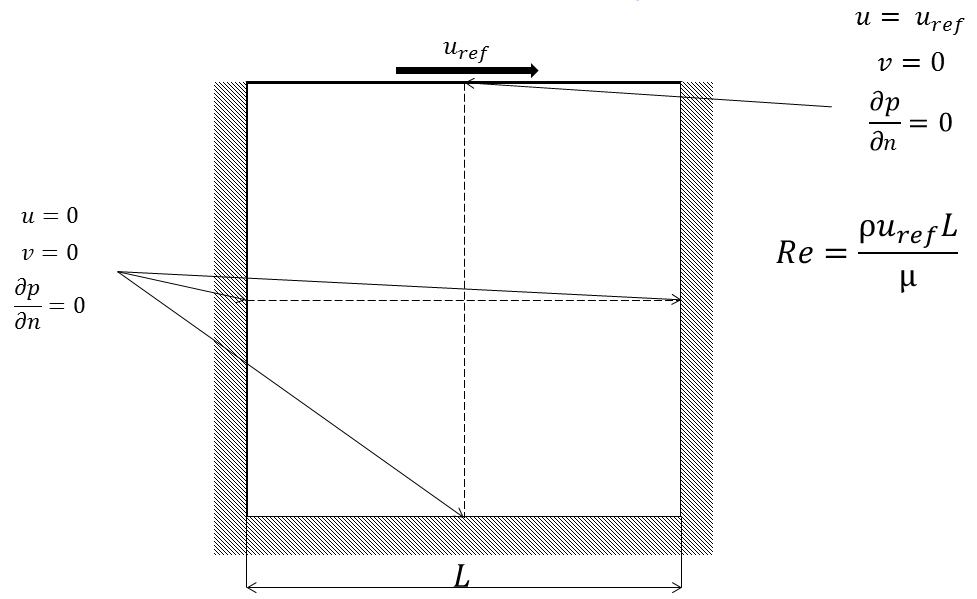
\includegraphics[scale=0.5]{DrivenCavity/DrivenCavity}
	\caption[General scheme of the driven cavity problem]{General scheme of the driven cavity problem. Extracted from \cite{CTTCa}}
	\label{DrivenCavityImg}
\end{figure}

\section{Discretization}
The domain is discretized, as explained in section \ref{FSMDiscretization}, using the staggered meshes. To do so, the volume is divided using a Cartesian grid, with the following characteristics:
\begin{table}[]
	\centering
	\begin{tabular}{ |c|c|c|c|c|c|c|c| }
		\hline
		$N$ & $M$ & $L$ & $\rho$ & $u_{ref}$ & $\mu$ & $Numerical scheme$ & $\delta$ \\ \hline
		$112$ & $112$ & $1$ & $1$ & $1$ & $\frac{1}{Re}$ & $CDS$ & $10^{-5}$ \\ \hline
	\end{tabular}
\caption{Numerical parameters of the driven cavity problem}
\end{table}

The length of the cavity $L$, the density $\rho$, the velocity $u_{ref}$ and the viscosity $\mu$ are chosen in order to have a non-dimensional problem. 

\section{Boundary conditions}
It is necessary to impose the conditions defined by figure \ref{DrivenCavityImg}. There are two types of conditions: the prescribed velocity, and the boundary layer conditions. The last ones are defined by assuming that the pressure gradient normal to the wall is 0. For example, in the left wall:
\begin{equation}
	\frac{\partial p}{\partial x}\approx\frac{p_{E}-p_{P}}{\Delta x}=0
\end{equation}
\begin{equation}
p_{P}=p_{E}
\end{equation}
These boundary layer conditions modify the discretization coefficients in the boundary nodes. The coefficients are listed in table \ref{DCBoundaryCoefficients}.
\begin{table}[h]
	\centering
	\begin{tabular}{ |c|c|c|c|c| }
		\hline
		Coefficients & Top & Bottom & Left & Right \\ \hline
		$a_{E}$ & 1 & 0 & 1 & 0 \\ \hline
		$a_{W}$ & 0 & 0 & 0 & 1 \\ \hline
		$a_{N}$ & 0 & 1 & 0 & 0 \\ \hline
		$a_{S}$ & 0 & 0 & 0 & 0 \\ \hline
		$a_{P}$ & 1 & 1 & 1 & 1 \\ \hline
	\end{tabular}
\caption{Discretization coefficients in the boundary}
\label{DCBoundaryCoefficients}
\end{table}

The condition of prescribed velocity in the walls is achieved with the following conditions:
\begin{itemize}
	\item $R\left(\vec{v}\right)=0$ in the top
	\item $R\left(\vec{v}\right)=0$ in the bottom wall
	\item $R\left(\vec{v}\right)=0$ in the left wall
	\item $R\left(\vec{v}\right)=0$ in the right wall
\end{itemize}
And the prescribed velocities are:
\begin{itemize}
	\item $u=u_{ref}$, $v=0$ in the top
	\item $u=0$, $v=0$ in the bottom wall
	\item $u=0$, $v=0$ in the left wall
	\item $u=0$, $v=0$ in the right wall
\end{itemize}

\section{Algorithm}
\begin{figure}[H]
	\centering
	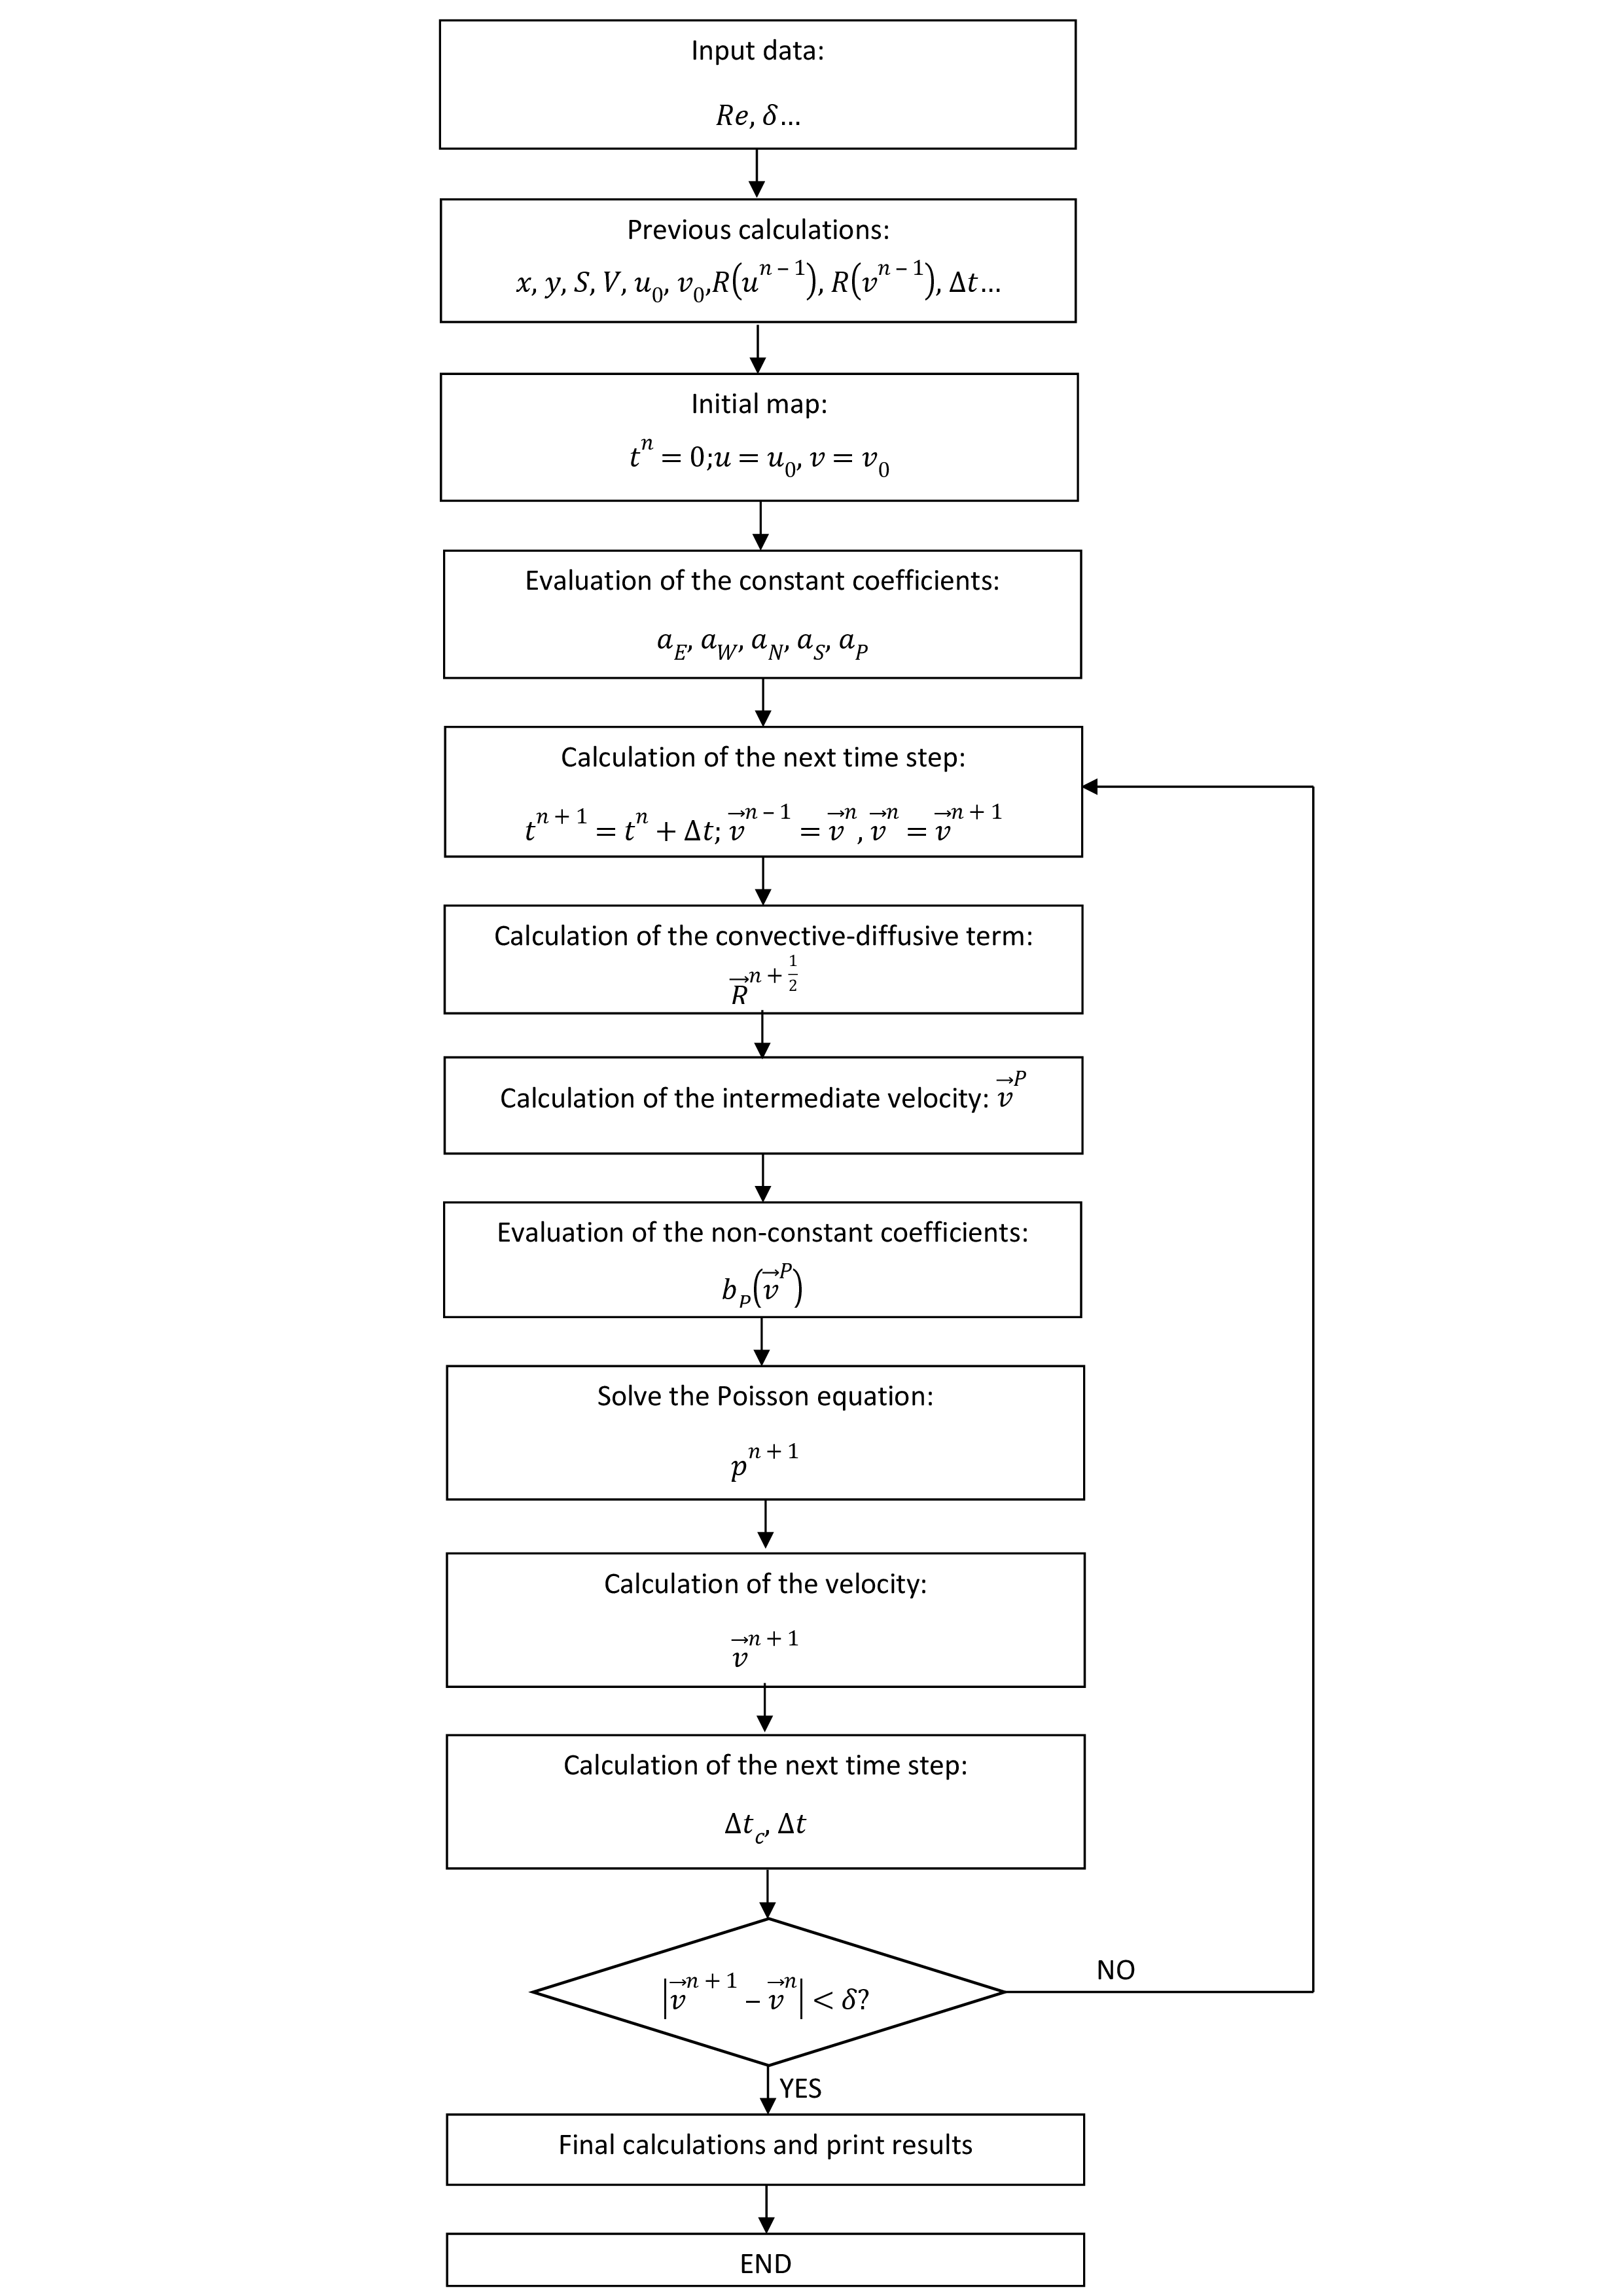
\includegraphics[scale=0.169]{DrivenCavity/algorithm}
\end{figure}
The simulation of the driven cavity problem ends when it reaches a steady state.

\section{Results}
In order to study the behaviour of the driven cavity problem in different ranges of flow, the simulation has been tested for $Re=100$, $400$, $1000$, $3200$, $5000$, $7500$ and $10000$. However not all cases are in the report; to see more results refer to Attachment A.

Figures \ref{Drivenhorizontal} and \ref{Drivenvertical} are a comparison between the obtained results and the reference ones for the velocities in the central planes. In both vertical and horizontal velocities, the best results are obtained for $Re=1000$. For low Reynolds the difference is slightly higher, but the results are still accurate. In the case of $Re=3200$ there is a point that presents a big error, but since it does not follow the distribution of the others it may be a typographical error. However, as the Reynolds increases, the error increases as well. In the cases of $Re\geq5000$, the results are rather different from the expected ones. Since these are high Reynolds, they may have not reached a steady state because they are turbulent.
\begin{figure}[h]
	\centering
	\begin{subfigure}{0.5\textwidth}
		\resizebox{1.4\textwidth}{!}{% GNUPLOT: LaTeX picture with Postscript
\begingroup
  \makeatletter
  \providecommand\color[2][]{%
    \GenericError{(gnuplot) \space\space\space\@spaces}{%
      Package color not loaded in conjunction with
      terminal option `colourtext'%
    }{See the gnuplot documentation for explanation.%
    }{Either use 'blacktext' in gnuplot or load the package
      color.sty in LaTeX.}%
    \renewcommand\color[2][]{}%
  }%
  \providecommand\includegraphics[2][]{%
    \GenericError{(gnuplot) \space\space\space\@spaces}{%
      Package graphicx or graphics not loaded%
    }{See the gnuplot documentation for explanation.%
    }{The gnuplot epslatex terminal needs graphicx.sty or graphics.sty.}%
    \renewcommand\includegraphics[2][]{}%
  }%
  \providecommand\rotatebox[2]{#2}%
  \@ifundefined{ifGPcolor}{%
    \newif\ifGPcolor
    \GPcolortrue
  }{}%
  \@ifundefined{ifGPblacktext}{%
    \newif\ifGPblacktext
    \GPblacktexttrue
  }{}%
  % define a \g@addto@macro without @ in the name:
  \let\gplgaddtomacro\g@addto@macro
  % define empty templates for all commands taking text:
  \gdef\gplbacktext{}%
  \gdef\gplfronttext{}%
  \makeatother
  \ifGPblacktext
    % no textcolor at all
    \def\colorrgb#1{}%
    \def\colorgray#1{}%
  \else
    % gray or color?
    \ifGPcolor
      \def\colorrgb#1{\color[rgb]{#1}}%
      \def\colorgray#1{\color[gray]{#1}}%
      \expandafter\def\csname LTw\endcsname{\color{white}}%
      \expandafter\def\csname LTb\endcsname{\color{black}}%
      \expandafter\def\csname LTa\endcsname{\color{black}}%
      \expandafter\def\csname LT0\endcsname{\color[rgb]{1,0,0}}%
      \expandafter\def\csname LT1\endcsname{\color[rgb]{0,1,0}}%
      \expandafter\def\csname LT2\endcsname{\color[rgb]{0,0,1}}%
      \expandafter\def\csname LT3\endcsname{\color[rgb]{1,0,1}}%
      \expandafter\def\csname LT4\endcsname{\color[rgb]{0,1,1}}%
      \expandafter\def\csname LT5\endcsname{\color[rgb]{1,1,0}}%
      \expandafter\def\csname LT6\endcsname{\color[rgb]{0,0,0}}%
      \expandafter\def\csname LT7\endcsname{\color[rgb]{1,0.3,0}}%
      \expandafter\def\csname LT8\endcsname{\color[rgb]{0.5,0.5,0.5}}%
    \else
      % gray
      \def\colorrgb#1{\color{black}}%
      \def\colorgray#1{\color[gray]{#1}}%
      \expandafter\def\csname LTw\endcsname{\color{white}}%
      \expandafter\def\csname LTb\endcsname{\color{black}}%
      \expandafter\def\csname LTa\endcsname{\color{black}}%
      \expandafter\def\csname LT0\endcsname{\color{black}}%
      \expandafter\def\csname LT1\endcsname{\color{black}}%
      \expandafter\def\csname LT2\endcsname{\color{black}}%
      \expandafter\def\csname LT3\endcsname{\color{black}}%
      \expandafter\def\csname LT4\endcsname{\color{black}}%
      \expandafter\def\csname LT5\endcsname{\color{black}}%
      \expandafter\def\csname LT6\endcsname{\color{black}}%
      \expandafter\def\csname LT7\endcsname{\color{black}}%
      \expandafter\def\csname LT8\endcsname{\color{black}}%
    \fi
  \fi
    \setlength{\unitlength}{0.0500bp}%
    \ifx\gptboxheight\undefined%
      \newlength{\gptboxheight}%
      \newlength{\gptboxwidth}%
      \newsavebox{\gptboxtext}%
    \fi%
    \setlength{\fboxrule}{0.5pt}%
    \setlength{\fboxsep}{1pt}%
\begin{picture}(7200.00,5040.00)%
    \gplgaddtomacro\gplbacktext{%
      \csname LTb\endcsname%
      \put(1487,484){\makebox(0,0)[r]{\strut{}$0$}}%
      \put(1487,1342){\makebox(0,0)[r]{\strut{}$0.2$}}%
      \put(1487,2200){\makebox(0,0)[r]{\strut{}$0.4$}}%
      \put(1487,3059){\makebox(0,0)[r]{\strut{}$0.6$}}%
      \put(1487,3917){\makebox(0,0)[r]{\strut{}$0.8$}}%
      \put(1487,4775){\makebox(0,0)[r]{\strut{}$1$}}%
      \put(1619,264){\makebox(0,0){\strut{}$-0.4$}}%
      \put(2232,264){\makebox(0,0){\strut{}$-0.2$}}%
      \put(2845,264){\makebox(0,0){\strut{}$0$}}%
      \put(3458,264){\makebox(0,0){\strut{}$0.2$}}%
      \put(4071,264){\makebox(0,0){\strut{}$0.4$}}%
      \put(4684,264){\makebox(0,0){\strut{}$0.6$}}%
      \put(5297,264){\makebox(0,0){\strut{}$0.8$}}%
      \put(5910,264){\makebox(0,0){\strut{}$1$}}%
    }%
    \gplgaddtomacro\gplfronttext{%
      \csname LTb\endcsname%
      \put(1245,4829){\makebox(0,0){\strut{}y}}%
      \put(3764,154){\makebox(0,0){\strut{}u}}%
      \csname LTb\endcsname%
      \put(3071,4602){\makebox(0,0)[r]{\strut{}Calculated}}%
      \csname LTb\endcsname%
      \put(3071,4382){\makebox(0,0)[r]{\strut{}Reference}}%
    }%
    \gplbacktext
    \put(0,0){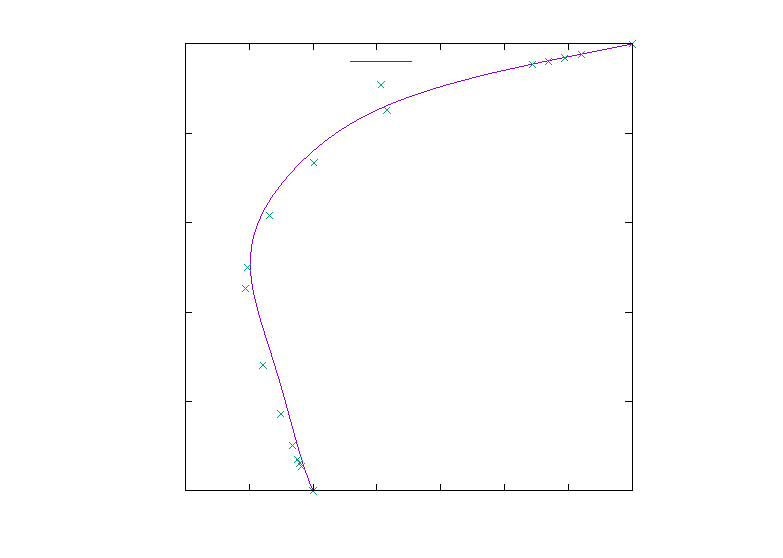
\includegraphics{DrivenCavity/u100}}%
    \gplfronttext
  \end{picture}%
\endgroup
}
		\caption{$Re=100$}
	\end{subfigure}%
	\begin{subfigure}{0.5\textwidth}
		\resizebox{1.4\textwidth}{!}{% GNUPLOT: LaTeX picture with Postscript
\begingroup
  \makeatletter
  \providecommand\color[2][]{%
    \GenericError{(gnuplot) \space\space\space\@spaces}{%
      Package color not loaded in conjunction with
      terminal option `colourtext'%
    }{See the gnuplot documentation for explanation.%
    }{Either use 'blacktext' in gnuplot or load the package
      color.sty in LaTeX.}%
    \renewcommand\color[2][]{}%
  }%
  \providecommand\includegraphics[2][]{%
    \GenericError{(gnuplot) \space\space\space\@spaces}{%
      Package graphicx or graphics not loaded%
    }{See the gnuplot documentation for explanation.%
    }{The gnuplot epslatex terminal needs graphicx.sty or graphics.sty.}%
    \renewcommand\includegraphics[2][]{}%
  }%
  \providecommand\rotatebox[2]{#2}%
  \@ifundefined{ifGPcolor}{%
    \newif\ifGPcolor
    \GPcolortrue
  }{}%
  \@ifundefined{ifGPblacktext}{%
    \newif\ifGPblacktext
    \GPblacktexttrue
  }{}%
  % define a \g@addto@macro without @ in the name:
  \let\gplgaddtomacro\g@addto@macro
  % define empty templates for all commands taking text:
  \gdef\gplbacktext{}%
  \gdef\gplfronttext{}%
  \makeatother
  \ifGPblacktext
    % no textcolor at all
    \def\colorrgb#1{}%
    \def\colorgray#1{}%
  \else
    % gray or color?
    \ifGPcolor
      \def\colorrgb#1{\color[rgb]{#1}}%
      \def\colorgray#1{\color[gray]{#1}}%
      \expandafter\def\csname LTw\endcsname{\color{white}}%
      \expandafter\def\csname LTb\endcsname{\color{black}}%
      \expandafter\def\csname LTa\endcsname{\color{black}}%
      \expandafter\def\csname LT0\endcsname{\color[rgb]{1,0,0}}%
      \expandafter\def\csname LT1\endcsname{\color[rgb]{0,1,0}}%
      \expandafter\def\csname LT2\endcsname{\color[rgb]{0,0,1}}%
      \expandafter\def\csname LT3\endcsname{\color[rgb]{1,0,1}}%
      \expandafter\def\csname LT4\endcsname{\color[rgb]{0,1,1}}%
      \expandafter\def\csname LT5\endcsname{\color[rgb]{1,1,0}}%
      \expandafter\def\csname LT6\endcsname{\color[rgb]{0,0,0}}%
      \expandafter\def\csname LT7\endcsname{\color[rgb]{1,0.3,0}}%
      \expandafter\def\csname LT8\endcsname{\color[rgb]{0.5,0.5,0.5}}%
    \else
      % gray
      \def\colorrgb#1{\color{black}}%
      \def\colorgray#1{\color[gray]{#1}}%
      \expandafter\def\csname LTw\endcsname{\color{white}}%
      \expandafter\def\csname LTb\endcsname{\color{black}}%
      \expandafter\def\csname LTa\endcsname{\color{black}}%
      \expandafter\def\csname LT0\endcsname{\color{black}}%
      \expandafter\def\csname LT1\endcsname{\color{black}}%
      \expandafter\def\csname LT2\endcsname{\color{black}}%
      \expandafter\def\csname LT3\endcsname{\color{black}}%
      \expandafter\def\csname LT4\endcsname{\color{black}}%
      \expandafter\def\csname LT5\endcsname{\color{black}}%
      \expandafter\def\csname LT6\endcsname{\color{black}}%
      \expandafter\def\csname LT7\endcsname{\color{black}}%
      \expandafter\def\csname LT8\endcsname{\color{black}}%
    \fi
  \fi
    \setlength{\unitlength}{0.0500bp}%
    \ifx\gptboxheight\undefined%
      \newlength{\gptboxheight}%
      \newlength{\gptboxwidth}%
      \newsavebox{\gptboxtext}%
    \fi%
    \setlength{\fboxrule}{0.5pt}%
    \setlength{\fboxsep}{1pt}%
\begin{picture}(7200.00,5040.00)%
    \gplgaddtomacro\gplbacktext{%
      \csname LTb\endcsname%
      \put(1531,440){\makebox(0,0)[r]{\strut{}$-0.4$}}%
      \put(1531,1059){\makebox(0,0)[r]{\strut{}$-0.2$}}%
      \put(1531,1679){\makebox(0,0)[r]{\strut{}$0$}}%
      \put(1531,2298){\makebox(0,0)[r]{\strut{}$0.2$}}%
      \put(1531,2917){\makebox(0,0)[r]{\strut{}$0.4$}}%
      \put(1531,3536){\makebox(0,0)[r]{\strut{}$0.6$}}%
      \put(1531,4156){\makebox(0,0)[r]{\strut{}$0.8$}}%
      \put(1531,4775){\makebox(0,0)[r]{\strut{}$1$}}%
      \put(1663,220){\makebox(0,0){\strut{}$0$}}%
      \put(2530,220){\makebox(0,0){\strut{}$0.2$}}%
      \put(3397,220){\makebox(0,0){\strut{}$0.4$}}%
      \put(4264,220){\makebox(0,0){\strut{}$0.6$}}%
      \put(5131,220){\makebox(0,0){\strut{}$0.8$}}%
      \put(5998,220){\makebox(0,0){\strut{}$1$}}%
    }%
    \gplgaddtomacro\gplfronttext{%
      \csname LTb\endcsname%
      \put(5011,4602){\makebox(0,0)[r]{\strut{}Calculated}}%
      \csname LTb\endcsname%
      \put(5011,4382){\makebox(0,0)[r]{\strut{}Reference}}%
    }%
    \gplbacktext
    \put(0,0){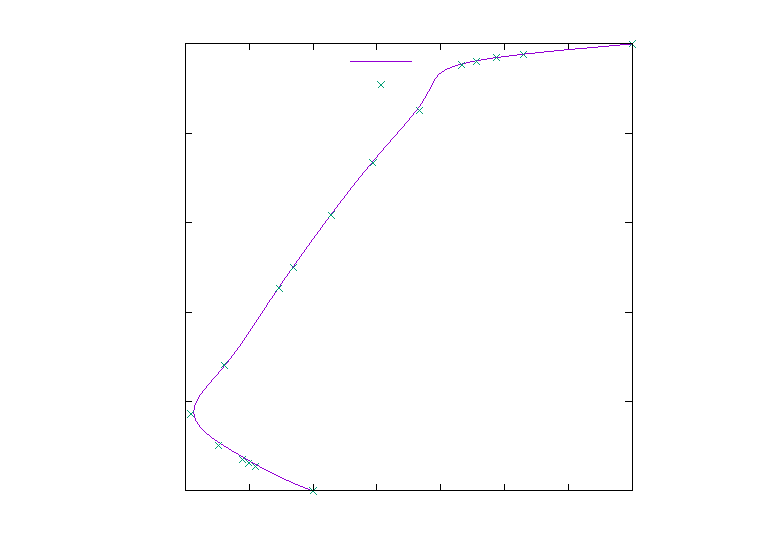
\includegraphics{u1000}}%
    \gplfronttext
  \end{picture}%
\endgroup
}
		\caption{$Re=1000$}
	\end{subfigure}
	\begin{subfigure}{0.5\textwidth}
		\resizebox{1.4\textwidth}{!}{% GNUPLOT: LaTeX picture with Postscript
\begingroup
  \makeatletter
  \providecommand\color[2][]{%
    \GenericError{(gnuplot) \space\space\space\@spaces}{%
      Package color not loaded in conjunction with
      terminal option `colourtext'%
    }{See the gnuplot documentation for explanation.%
    }{Either use 'blacktext' in gnuplot or load the package
      color.sty in LaTeX.}%
    \renewcommand\color[2][]{}%
  }%
  \providecommand\includegraphics[2][]{%
    \GenericError{(gnuplot) \space\space\space\@spaces}{%
      Package graphicx or graphics not loaded%
    }{See the gnuplot documentation for explanation.%
    }{The gnuplot epslatex terminal needs graphicx.sty or graphics.sty.}%
    \renewcommand\includegraphics[2][]{}%
  }%
  \providecommand\rotatebox[2]{#2}%
  \@ifundefined{ifGPcolor}{%
    \newif\ifGPcolor
    \GPcolortrue
  }{}%
  \@ifundefined{ifGPblacktext}{%
    \newif\ifGPblacktext
    \GPblacktexttrue
  }{}%
  % define a \g@addto@macro without @ in the name:
  \let\gplgaddtomacro\g@addto@macro
  % define empty templates for all commands taking text:
  \gdef\gplbacktext{}%
  \gdef\gplfronttext{}%
  \makeatother
  \ifGPblacktext
    % no textcolor at all
    \def\colorrgb#1{}%
    \def\colorgray#1{}%
  \else
    % gray or color?
    \ifGPcolor
      \def\colorrgb#1{\color[rgb]{#1}}%
      \def\colorgray#1{\color[gray]{#1}}%
      \expandafter\def\csname LTw\endcsname{\color{white}}%
      \expandafter\def\csname LTb\endcsname{\color{black}}%
      \expandafter\def\csname LTa\endcsname{\color{black}}%
      \expandafter\def\csname LT0\endcsname{\color[rgb]{1,0,0}}%
      \expandafter\def\csname LT1\endcsname{\color[rgb]{0,1,0}}%
      \expandafter\def\csname LT2\endcsname{\color[rgb]{0,0,1}}%
      \expandafter\def\csname LT3\endcsname{\color[rgb]{1,0,1}}%
      \expandafter\def\csname LT4\endcsname{\color[rgb]{0,1,1}}%
      \expandafter\def\csname LT5\endcsname{\color[rgb]{1,1,0}}%
      \expandafter\def\csname LT6\endcsname{\color[rgb]{0,0,0}}%
      \expandafter\def\csname LT7\endcsname{\color[rgb]{1,0.3,0}}%
      \expandafter\def\csname LT8\endcsname{\color[rgb]{0.5,0.5,0.5}}%
    \else
      % gray
      \def\colorrgb#1{\color{black}}%
      \def\colorgray#1{\color[gray]{#1}}%
      \expandafter\def\csname LTw\endcsname{\color{white}}%
      \expandafter\def\csname LTb\endcsname{\color{black}}%
      \expandafter\def\csname LTa\endcsname{\color{black}}%
      \expandafter\def\csname LT0\endcsname{\color{black}}%
      \expandafter\def\csname LT1\endcsname{\color{black}}%
      \expandafter\def\csname LT2\endcsname{\color{black}}%
      \expandafter\def\csname LT3\endcsname{\color{black}}%
      \expandafter\def\csname LT4\endcsname{\color{black}}%
      \expandafter\def\csname LT5\endcsname{\color{black}}%
      \expandafter\def\csname LT6\endcsname{\color{black}}%
      \expandafter\def\csname LT7\endcsname{\color{black}}%
      \expandafter\def\csname LT8\endcsname{\color{black}}%
    \fi
  \fi
    \setlength{\unitlength}{0.0500bp}%
    \ifx\gptboxheight\undefined%
      \newlength{\gptboxheight}%
      \newlength{\gptboxwidth}%
      \newsavebox{\gptboxtext}%
    \fi%
    \setlength{\fboxrule}{0.5pt}%
    \setlength{\fboxsep}{1pt}%
\begin{picture}(7200.00,5040.00)%
    \gplgaddtomacro\gplbacktext{%
      \csname LTb\endcsname%
      \put(1531,440){\makebox(0,0)[r]{\strut{}$-1$}}%
      \put(1531,873){\makebox(0,0)[r]{\strut{}$-0.8$}}%
      \put(1531,1307){\makebox(0,0)[r]{\strut{}$-0.6$}}%
      \put(1531,1740){\makebox(0,0)[r]{\strut{}$-0.4$}}%
      \put(1531,2174){\makebox(0,0)[r]{\strut{}$-0.2$}}%
      \put(1531,2608){\makebox(0,0)[r]{\strut{}$0$}}%
      \put(1531,3041){\makebox(0,0)[r]{\strut{}$0.2$}}%
      \put(1531,3475){\makebox(0,0)[r]{\strut{}$0.4$}}%
      \put(1531,3908){\makebox(0,0)[r]{\strut{}$0.6$}}%
      \put(1531,4342){\makebox(0,0)[r]{\strut{}$0.8$}}%
      \put(1531,4775){\makebox(0,0)[r]{\strut{}$1$}}%
      \put(1663,220){\makebox(0,0){\strut{}$0$}}%
      \put(2530,220){\makebox(0,0){\strut{}$0.2$}}%
      \put(3397,220){\makebox(0,0){\strut{}$0.4$}}%
      \put(4264,220){\makebox(0,0){\strut{}$0.6$}}%
      \put(5131,220){\makebox(0,0){\strut{}$0.8$}}%
      \put(5998,220){\makebox(0,0){\strut{}$1$}}%
    }%
    \gplgaddtomacro\gplfronttext{%
      \csname LTb\endcsname%
      \put(5011,4602){\makebox(0,0)[r]{\strut{}Calculated}}%
      \csname LTb\endcsname%
      \put(5011,4382){\makebox(0,0)[r]{\strut{}Reference}}%
    }%
    \gplbacktext
    \put(0,0){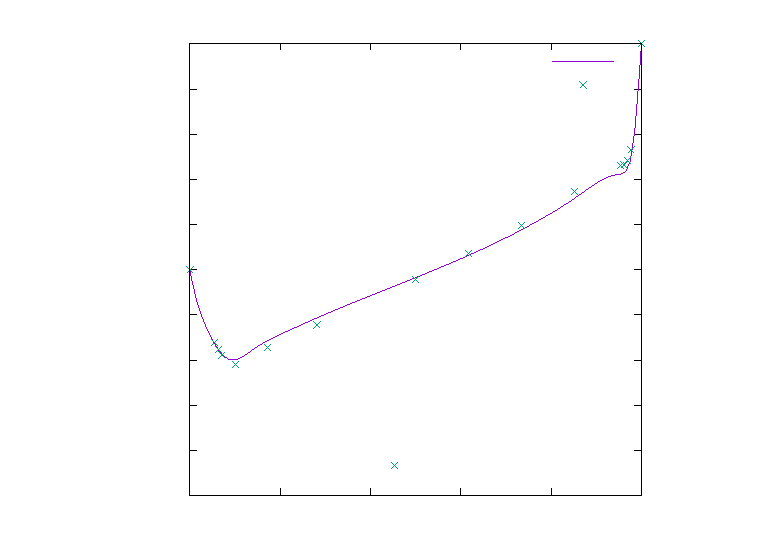
\includegraphics{u3200}}%
    \gplfronttext
  \end{picture}%
\endgroup
}
		\caption{$Re=3200$}
	\end{subfigure}%
	\begin{subfigure}{0.5\textwidth}
		\center
		\resizebox{1.4\textwidth}{!}{% GNUPLOT: LaTeX picture with Postscript
\begingroup
  \makeatletter
  \providecommand\color[2][]{%
    \GenericError{(gnuplot) \space\space\space\@spaces}{%
      Package color not loaded in conjunction with
      terminal option `colourtext'%
    }{See the gnuplot documentation for explanation.%
    }{Either use 'blacktext' in gnuplot or load the package
      color.sty in LaTeX.}%
    \renewcommand\color[2][]{}%
  }%
  \providecommand\includegraphics[2][]{%
    \GenericError{(gnuplot) \space\space\space\@spaces}{%
      Package graphicx or graphics not loaded%
    }{See the gnuplot documentation for explanation.%
    }{The gnuplot epslatex terminal needs graphicx.sty or graphics.sty.}%
    \renewcommand\includegraphics[2][]{}%
  }%
  \providecommand\rotatebox[2]{#2}%
  \@ifundefined{ifGPcolor}{%
    \newif\ifGPcolor
    \GPcolortrue
  }{}%
  \@ifundefined{ifGPblacktext}{%
    \newif\ifGPblacktext
    \GPblacktexttrue
  }{}%
  % define a \g@addto@macro without @ in the name:
  \let\gplgaddtomacro\g@addto@macro
  % define empty templates for all commands taking text:
  \gdef\gplbacktext{}%
  \gdef\gplfronttext{}%
  \makeatother
  \ifGPblacktext
    % no textcolor at all
    \def\colorrgb#1{}%
    \def\colorgray#1{}%
  \else
    % gray or color?
    \ifGPcolor
      \def\colorrgb#1{\color[rgb]{#1}}%
      \def\colorgray#1{\color[gray]{#1}}%
      \expandafter\def\csname LTw\endcsname{\color{white}}%
      \expandafter\def\csname LTb\endcsname{\color{black}}%
      \expandafter\def\csname LTa\endcsname{\color{black}}%
      \expandafter\def\csname LT0\endcsname{\color[rgb]{1,0,0}}%
      \expandafter\def\csname LT1\endcsname{\color[rgb]{0,1,0}}%
      \expandafter\def\csname LT2\endcsname{\color[rgb]{0,0,1}}%
      \expandafter\def\csname LT3\endcsname{\color[rgb]{1,0,1}}%
      \expandafter\def\csname LT4\endcsname{\color[rgb]{0,1,1}}%
      \expandafter\def\csname LT5\endcsname{\color[rgb]{1,1,0}}%
      \expandafter\def\csname LT6\endcsname{\color[rgb]{0,0,0}}%
      \expandafter\def\csname LT7\endcsname{\color[rgb]{1,0.3,0}}%
      \expandafter\def\csname LT8\endcsname{\color[rgb]{0.5,0.5,0.5}}%
    \else
      % gray
      \def\colorrgb#1{\color{black}}%
      \def\colorgray#1{\color[gray]{#1}}%
      \expandafter\def\csname LTw\endcsname{\color{white}}%
      \expandafter\def\csname LTb\endcsname{\color{black}}%
      \expandafter\def\csname LTa\endcsname{\color{black}}%
      \expandafter\def\csname LT0\endcsname{\color{black}}%
      \expandafter\def\csname LT1\endcsname{\color{black}}%
      \expandafter\def\csname LT2\endcsname{\color{black}}%
      \expandafter\def\csname LT3\endcsname{\color{black}}%
      \expandafter\def\csname LT4\endcsname{\color{black}}%
      \expandafter\def\csname LT5\endcsname{\color{black}}%
      \expandafter\def\csname LT6\endcsname{\color{black}}%
      \expandafter\def\csname LT7\endcsname{\color{black}}%
      \expandafter\def\csname LT8\endcsname{\color{black}}%
    \fi
  \fi
    \setlength{\unitlength}{0.0500bp}%
    \ifx\gptboxheight\undefined%
      \newlength{\gptboxheight}%
      \newlength{\gptboxwidth}%
      \newsavebox{\gptboxtext}%
    \fi%
    \setlength{\fboxrule}{0.5pt}%
    \setlength{\fboxsep}{1pt}%
\begin{picture}(7200.00,5040.00)%
    \gplgaddtomacro\gplbacktext{%
      \csname LTb\endcsname%
      \put(1531,440){\makebox(0,0)[r]{\strut{}$-0.6$}}%
      \put(1531,982){\makebox(0,0)[r]{\strut{}$-0.4$}}%
      \put(1531,1524){\makebox(0,0)[r]{\strut{}$-0.2$}}%
      \put(1531,2066){\makebox(0,0)[r]{\strut{}$0$}}%
      \put(1531,2608){\makebox(0,0)[r]{\strut{}$0.2$}}%
      \put(1531,3149){\makebox(0,0)[r]{\strut{}$0.4$}}%
      \put(1531,3691){\makebox(0,0)[r]{\strut{}$0.6$}}%
      \put(1531,4233){\makebox(0,0)[r]{\strut{}$0.8$}}%
      \put(1531,4775){\makebox(0,0)[r]{\strut{}$1$}}%
      \put(1663,220){\makebox(0,0){\strut{}$0$}}%
      \put(2530,220){\makebox(0,0){\strut{}$0.2$}}%
      \put(3397,220){\makebox(0,0){\strut{}$0.4$}}%
      \put(4264,220){\makebox(0,0){\strut{}$0.6$}}%
      \put(5131,220){\makebox(0,0){\strut{}$0.8$}}%
      \put(5998,220){\makebox(0,0){\strut{}$1$}}%
    }%
    \gplgaddtomacro\gplfronttext{%
      \csname LTb\endcsname%
      \put(5011,4602){\makebox(0,0)[r]{\strut{}Calculated}}%
      \csname LTb\endcsname%
      \put(5011,4382){\makebox(0,0)[r]{\strut{}Reference}}%
    }%
    \gplbacktext
    \put(0,0){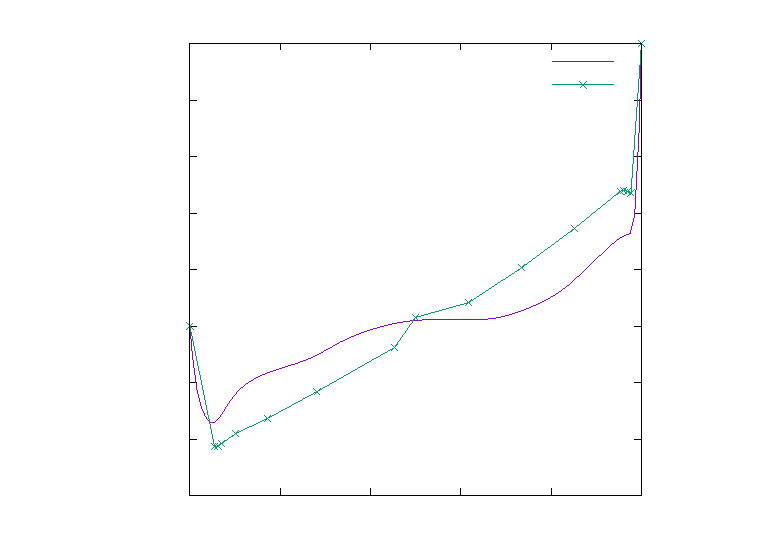
\includegraphics{u10000}}%
    \gplfronttext
  \end{picture}%
\endgroup
}
		\caption{$Re=10000$}
	\end{subfigure}
	\caption[Comparison between the reference solution and the calculated one of the horizontal velocity along the vertical line in the geometric center of the cavity]{Comparison between the reference solution and the calculated one of the horizontal velocity along the vertical line in the geometric centre of the cavity \cite{Ghia1982}}
	\label{Drivenhorizontal}
\end{figure}

\begin{figure}[h]
	\centering
	\begin{subfigure}{0.5\textwidth}
		\resizebox{1.4\textwidth}{!}{% GNUPLOT: LaTeX picture with Postscript
\begingroup
  \makeatletter
  \providecommand\color[2][]{%
    \GenericError{(gnuplot) \space\space\space\@spaces}{%
      Package color not loaded in conjunction with
      terminal option `colourtext'%
    }{See the gnuplot documentation for explanation.%
    }{Either use 'blacktext' in gnuplot or load the package
      color.sty in LaTeX.}%
    \renewcommand\color[2][]{}%
  }%
  \providecommand\includegraphics[2][]{%
    \GenericError{(gnuplot) \space\space\space\@spaces}{%
      Package graphicx or graphics not loaded%
    }{See the gnuplot documentation for explanation.%
    }{The gnuplot epslatex terminal needs graphicx.sty or graphics.sty.}%
    \renewcommand\includegraphics[2][]{}%
  }%
  \providecommand\rotatebox[2]{#2}%
  \@ifundefined{ifGPcolor}{%
    \newif\ifGPcolor
    \GPcolortrue
  }{}%
  \@ifundefined{ifGPblacktext}{%
    \newif\ifGPblacktext
    \GPblacktexttrue
  }{}%
  % define a \g@addto@macro without @ in the name:
  \let\gplgaddtomacro\g@addto@macro
  % define empty templates for all commands taking text:
  \gdef\gplbacktext{}%
  \gdef\gplfronttext{}%
  \makeatother
  \ifGPblacktext
    % no textcolor at all
    \def\colorrgb#1{}%
    \def\colorgray#1{}%
  \else
    % gray or color?
    \ifGPcolor
      \def\colorrgb#1{\color[rgb]{#1}}%
      \def\colorgray#1{\color[gray]{#1}}%
      \expandafter\def\csname LTw\endcsname{\color{white}}%
      \expandafter\def\csname LTb\endcsname{\color{black}}%
      \expandafter\def\csname LTa\endcsname{\color{black}}%
      \expandafter\def\csname LT0\endcsname{\color[rgb]{1,0,0}}%
      \expandafter\def\csname LT1\endcsname{\color[rgb]{0,1,0}}%
      \expandafter\def\csname LT2\endcsname{\color[rgb]{0,0,1}}%
      \expandafter\def\csname LT3\endcsname{\color[rgb]{1,0,1}}%
      \expandafter\def\csname LT4\endcsname{\color[rgb]{0,1,1}}%
      \expandafter\def\csname LT5\endcsname{\color[rgb]{1,1,0}}%
      \expandafter\def\csname LT6\endcsname{\color[rgb]{0,0,0}}%
      \expandafter\def\csname LT7\endcsname{\color[rgb]{1,0.3,0}}%
      \expandafter\def\csname LT8\endcsname{\color[rgb]{0.5,0.5,0.5}}%
    \else
      % gray
      \def\colorrgb#1{\color{black}}%
      \def\colorgray#1{\color[gray]{#1}}%
      \expandafter\def\csname LTw\endcsname{\color{white}}%
      \expandafter\def\csname LTb\endcsname{\color{black}}%
      \expandafter\def\csname LTa\endcsname{\color{black}}%
      \expandafter\def\csname LT0\endcsname{\color{black}}%
      \expandafter\def\csname LT1\endcsname{\color{black}}%
      \expandafter\def\csname LT2\endcsname{\color{black}}%
      \expandafter\def\csname LT3\endcsname{\color{black}}%
      \expandafter\def\csname LT4\endcsname{\color{black}}%
      \expandafter\def\csname LT5\endcsname{\color{black}}%
      \expandafter\def\csname LT6\endcsname{\color{black}}%
      \expandafter\def\csname LT7\endcsname{\color{black}}%
      \expandafter\def\csname LT8\endcsname{\color{black}}%
    \fi
  \fi
    \setlength{\unitlength}{0.0500bp}%
    \ifx\gptboxheight\undefined%
      \newlength{\gptboxheight}%
      \newlength{\gptboxwidth}%
      \newsavebox{\gptboxtext}%
    \fi%
    \setlength{\fboxrule}{0.5pt}%
    \setlength{\fboxsep}{1pt}%
\begin{picture}(7200.00,5040.00)%
    \gplgaddtomacro\gplbacktext{%
      \csname LTb\endcsname%
      \put(1619,484){\makebox(0,0)[r]{\strut{}$-0.25$}}%
      \put(1619,961){\makebox(0,0)[r]{\strut{}$-0.2$}}%
      \put(1619,1438){\makebox(0,0)[r]{\strut{}$-0.15$}}%
      \put(1619,1914){\makebox(0,0)[r]{\strut{}$-0.1$}}%
      \put(1619,2391){\makebox(0,0)[r]{\strut{}$-0.05$}}%
      \put(1619,2868){\makebox(0,0)[r]{\strut{}$0$}}%
      \put(1619,3345){\makebox(0,0)[r]{\strut{}$0.05$}}%
      \put(1619,3821){\makebox(0,0)[r]{\strut{}$0.1$}}%
      \put(1619,4298){\makebox(0,0)[r]{\strut{}$0.15$}}%
      \put(1619,4775){\makebox(0,0)[r]{\strut{}$0.2$}}%
      \put(1751,264){\makebox(0,0){\strut{}$0$}}%
      \put(2609,264){\makebox(0,0){\strut{}$0.2$}}%
      \put(3467,264){\makebox(0,0){\strut{}$0.4$}}%
      \put(4326,264){\makebox(0,0){\strut{}$0.6$}}%
      \put(5184,264){\makebox(0,0){\strut{}$0.8$}}%
      \put(6042,264){\makebox(0,0){\strut{}$1$}}%
    }%
    \gplgaddtomacro\gplfronttext{%
      \csname LTb\endcsname%
      \put(1113,4829){\makebox(0,0){\strut{}v}}%
      \put(3896,154){\makebox(0,0){\strut{}x}}%
      \csname LTb\endcsname%
      \put(5055,4602){\makebox(0,0)[r]{\strut{}Calculated}}%
      \csname LTb\endcsname%
      \put(5055,4382){\makebox(0,0)[r]{\strut{}Reference}}%
    }%
    \gplbacktext
    \put(0,0){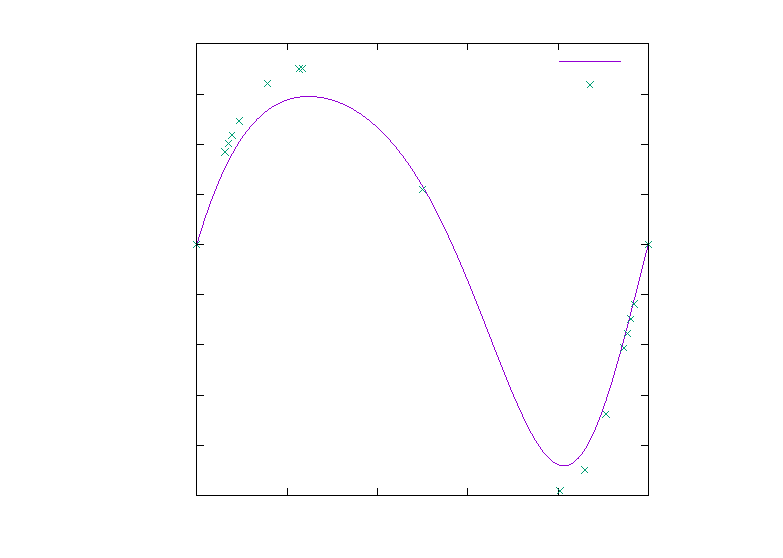
\includegraphics{DrivenCavity/v100}}%
    \gplfronttext
  \end{picture}%
\endgroup
}
		\caption{$Re=100$}
	\end{subfigure}%
	\begin{subfigure}{0.5\textwidth}
		\resizebox{1.4\textwidth}{!}{% GNUPLOT: LaTeX picture with Postscript
\begingroup
  \makeatletter
  \providecommand\color[2][]{%
    \GenericError{(gnuplot) \space\space\space\@spaces}{%
      Package color not loaded in conjunction with
      terminal option `colourtext'%
    }{See the gnuplot documentation for explanation.%
    }{Either use 'blacktext' in gnuplot or load the package
      color.sty in LaTeX.}%
    \renewcommand\color[2][]{}%
  }%
  \providecommand\includegraphics[2][]{%
    \GenericError{(gnuplot) \space\space\space\@spaces}{%
      Package graphicx or graphics not loaded%
    }{See the gnuplot documentation for explanation.%
    }{The gnuplot epslatex terminal needs graphicx.sty or graphics.sty.}%
    \renewcommand\includegraphics[2][]{}%
  }%
  \providecommand\rotatebox[2]{#2}%
  \@ifundefined{ifGPcolor}{%
    \newif\ifGPcolor
    \GPcolortrue
  }{}%
  \@ifundefined{ifGPblacktext}{%
    \newif\ifGPblacktext
    \GPblacktexttrue
  }{}%
  % define a \g@addto@macro without @ in the name:
  \let\gplgaddtomacro\g@addto@macro
  % define empty templates for all commands taking text:
  \gdef\gplbacktext{}%
  \gdef\gplfronttext{}%
  \makeatother
  \ifGPblacktext
    % no textcolor at all
    \def\colorrgb#1{}%
    \def\colorgray#1{}%
  \else
    % gray or color?
    \ifGPcolor
      \def\colorrgb#1{\color[rgb]{#1}}%
      \def\colorgray#1{\color[gray]{#1}}%
      \expandafter\def\csname LTw\endcsname{\color{white}}%
      \expandafter\def\csname LTb\endcsname{\color{black}}%
      \expandafter\def\csname LTa\endcsname{\color{black}}%
      \expandafter\def\csname LT0\endcsname{\color[rgb]{1,0,0}}%
      \expandafter\def\csname LT1\endcsname{\color[rgb]{0,1,0}}%
      \expandafter\def\csname LT2\endcsname{\color[rgb]{0,0,1}}%
      \expandafter\def\csname LT3\endcsname{\color[rgb]{1,0,1}}%
      \expandafter\def\csname LT4\endcsname{\color[rgb]{0,1,1}}%
      \expandafter\def\csname LT5\endcsname{\color[rgb]{1,1,0}}%
      \expandafter\def\csname LT6\endcsname{\color[rgb]{0,0,0}}%
      \expandafter\def\csname LT7\endcsname{\color[rgb]{1,0.3,0}}%
      \expandafter\def\csname LT8\endcsname{\color[rgb]{0.5,0.5,0.5}}%
    \else
      % gray
      \def\colorrgb#1{\color{black}}%
      \def\colorgray#1{\color[gray]{#1}}%
      \expandafter\def\csname LTw\endcsname{\color{white}}%
      \expandafter\def\csname LTb\endcsname{\color{black}}%
      \expandafter\def\csname LTa\endcsname{\color{black}}%
      \expandafter\def\csname LT0\endcsname{\color{black}}%
      \expandafter\def\csname LT1\endcsname{\color{black}}%
      \expandafter\def\csname LT2\endcsname{\color{black}}%
      \expandafter\def\csname LT3\endcsname{\color{black}}%
      \expandafter\def\csname LT4\endcsname{\color{black}}%
      \expandafter\def\csname LT5\endcsname{\color{black}}%
      \expandafter\def\csname LT6\endcsname{\color{black}}%
      \expandafter\def\csname LT7\endcsname{\color{black}}%
      \expandafter\def\csname LT8\endcsname{\color{black}}%
    \fi
  \fi
    \setlength{\unitlength}{0.0500bp}%
    \ifx\gptboxheight\undefined%
      \newlength{\gptboxheight}%
      \newlength{\gptboxwidth}%
      \newsavebox{\gptboxtext}%
    \fi%
    \setlength{\fboxrule}{0.5pt}%
    \setlength{\fboxsep}{1pt}%
\begin{picture}(7200.00,5040.00)%
    \gplgaddtomacro\gplbacktext{%
      \csname LTb\endcsname%
      \put(1531,440){\makebox(0,0)[r]{\strut{}$-0.6$}}%
      \put(1531,873){\makebox(0,0)[r]{\strut{}$-0.5$}}%
      \put(1531,1307){\makebox(0,0)[r]{\strut{}$-0.4$}}%
      \put(1531,1740){\makebox(0,0)[r]{\strut{}$-0.3$}}%
      \put(1531,2174){\makebox(0,0)[r]{\strut{}$-0.2$}}%
      \put(1531,2607){\makebox(0,0)[r]{\strut{}$-0.1$}}%
      \put(1531,3041){\makebox(0,0)[r]{\strut{}$0$}}%
      \put(1531,3475){\makebox(0,0)[r]{\strut{}$0.1$}}%
      \put(1531,3908){\makebox(0,0)[r]{\strut{}$0.2$}}%
      \put(1531,4342){\makebox(0,0)[r]{\strut{}$0.3$}}%
      \put(1531,4775){\makebox(0,0)[r]{\strut{}$0.4$}}%
      \put(1663,220){\makebox(0,0){\strut{}$0$}}%
      \put(2530,220){\makebox(0,0){\strut{}$0.2$}}%
      \put(3397,220){\makebox(0,0){\strut{}$0.4$}}%
      \put(4264,220){\makebox(0,0){\strut{}$0.6$}}%
      \put(5131,220){\makebox(0,0){\strut{}$0.8$}}%
      \put(5998,220){\makebox(0,0){\strut{}$1$}}%
    }%
    \gplgaddtomacro\gplfronttext{%
      \csname LTb\endcsname%
      \put(5011,4602){\makebox(0,0)[r]{\strut{}Calculated}}%
      \csname LTb\endcsname%
      \put(5011,4382){\makebox(0,0)[r]{\strut{}Reference}}%
    }%
    \gplbacktext
    \put(0,0){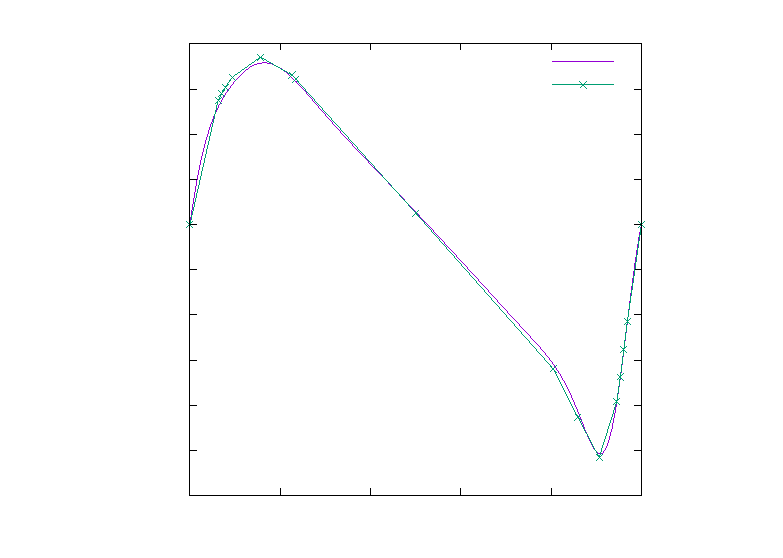
\includegraphics{v1000}}%
    \gplfronttext
  \end{picture}%
\endgroup
}
		\caption{$Re=1000$}
	\end{subfigure}
	\begin{subfigure}{0.5\textwidth}
		\resizebox{1.4\textwidth}{!}{% GNUPLOT: LaTeX picture with Postscript
\begingroup
  \makeatletter
  \providecommand\color[2][]{%
    \GenericError{(gnuplot) \space\space\space\@spaces}{%
      Package color not loaded in conjunction with
      terminal option `colourtext'%
    }{See the gnuplot documentation for explanation.%
    }{Either use 'blacktext' in gnuplot or load the package
      color.sty in LaTeX.}%
    \renewcommand\color[2][]{}%
  }%
  \providecommand\includegraphics[2][]{%
    \GenericError{(gnuplot) \space\space\space\@spaces}{%
      Package graphicx or graphics not loaded%
    }{See the gnuplot documentation for explanation.%
    }{The gnuplot epslatex terminal needs graphicx.sty or graphics.sty.}%
    \renewcommand\includegraphics[2][]{}%
  }%
  \providecommand\rotatebox[2]{#2}%
  \@ifundefined{ifGPcolor}{%
    \newif\ifGPcolor
    \GPcolortrue
  }{}%
  \@ifundefined{ifGPblacktext}{%
    \newif\ifGPblacktext
    \GPblacktexttrue
  }{}%
  % define a \g@addto@macro without @ in the name:
  \let\gplgaddtomacro\g@addto@macro
  % define empty templates for all commands taking text:
  \gdef\gplbacktext{}%
  \gdef\gplfronttext{}%
  \makeatother
  \ifGPblacktext
    % no textcolor at all
    \def\colorrgb#1{}%
    \def\colorgray#1{}%
  \else
    % gray or color?
    \ifGPcolor
      \def\colorrgb#1{\color[rgb]{#1}}%
      \def\colorgray#1{\color[gray]{#1}}%
      \expandafter\def\csname LTw\endcsname{\color{white}}%
      \expandafter\def\csname LTb\endcsname{\color{black}}%
      \expandafter\def\csname LTa\endcsname{\color{black}}%
      \expandafter\def\csname LT0\endcsname{\color[rgb]{1,0,0}}%
      \expandafter\def\csname LT1\endcsname{\color[rgb]{0,1,0}}%
      \expandafter\def\csname LT2\endcsname{\color[rgb]{0,0,1}}%
      \expandafter\def\csname LT3\endcsname{\color[rgb]{1,0,1}}%
      \expandafter\def\csname LT4\endcsname{\color[rgb]{0,1,1}}%
      \expandafter\def\csname LT5\endcsname{\color[rgb]{1,1,0}}%
      \expandafter\def\csname LT6\endcsname{\color[rgb]{0,0,0}}%
      \expandafter\def\csname LT7\endcsname{\color[rgb]{1,0.3,0}}%
      \expandafter\def\csname LT8\endcsname{\color[rgb]{0.5,0.5,0.5}}%
    \else
      % gray
      \def\colorrgb#1{\color{black}}%
      \def\colorgray#1{\color[gray]{#1}}%
      \expandafter\def\csname LTw\endcsname{\color{white}}%
      \expandafter\def\csname LTb\endcsname{\color{black}}%
      \expandafter\def\csname LTa\endcsname{\color{black}}%
      \expandafter\def\csname LT0\endcsname{\color{black}}%
      \expandafter\def\csname LT1\endcsname{\color{black}}%
      \expandafter\def\csname LT2\endcsname{\color{black}}%
      \expandafter\def\csname LT3\endcsname{\color{black}}%
      \expandafter\def\csname LT4\endcsname{\color{black}}%
      \expandafter\def\csname LT5\endcsname{\color{black}}%
      \expandafter\def\csname LT6\endcsname{\color{black}}%
      \expandafter\def\csname LT7\endcsname{\color{black}}%
      \expandafter\def\csname LT8\endcsname{\color{black}}%
    \fi
  \fi
    \setlength{\unitlength}{0.0500bp}%
    \ifx\gptboxheight\undefined%
      \newlength{\gptboxheight}%
      \newlength{\gptboxwidth}%
      \newsavebox{\gptboxtext}%
    \fi%
    \setlength{\fboxrule}{0.5pt}%
    \setlength{\fboxsep}{1pt}%
\begin{picture}(7200.00,5040.00)%
    \gplgaddtomacro\gplbacktext{%
      \csname LTb\endcsname%
      \put(1531,440){\makebox(0,0)[r]{\strut{}$-0.6$}}%
      \put(1531,834){\makebox(0,0)[r]{\strut{}$-0.5$}}%
      \put(1531,1228){\makebox(0,0)[r]{\strut{}$-0.4$}}%
      \put(1531,1622){\makebox(0,0)[r]{\strut{}$-0.3$}}%
      \put(1531,2016){\makebox(0,0)[r]{\strut{}$-0.2$}}%
      \put(1531,2410){\makebox(0,0)[r]{\strut{}$-0.1$}}%
      \put(1531,2805){\makebox(0,0)[r]{\strut{}$0$}}%
      \put(1531,3199){\makebox(0,0)[r]{\strut{}$0.1$}}%
      \put(1531,3593){\makebox(0,0)[r]{\strut{}$0.2$}}%
      \put(1531,3987){\makebox(0,0)[r]{\strut{}$0.3$}}%
      \put(1531,4381){\makebox(0,0)[r]{\strut{}$0.4$}}%
      \put(1531,4775){\makebox(0,0)[r]{\strut{}$0.5$}}%
      \put(1663,220){\makebox(0,0){\strut{}$0$}}%
      \put(2530,220){\makebox(0,0){\strut{}$0.2$}}%
      \put(3397,220){\makebox(0,0){\strut{}$0.4$}}%
      \put(4264,220){\makebox(0,0){\strut{}$0.6$}}%
      \put(5131,220){\makebox(0,0){\strut{}$0.8$}}%
      \put(5998,220){\makebox(0,0){\strut{}$1$}}%
    }%
    \gplgaddtomacro\gplfronttext{%
      \csname LTb\endcsname%
      \put(5011,4602){\makebox(0,0)[r]{\strut{}Calculated}}%
      \csname LTb\endcsname%
      \put(5011,4382){\makebox(0,0)[r]{\strut{}Reference}}%
    }%
    \gplbacktext
    \put(0,0){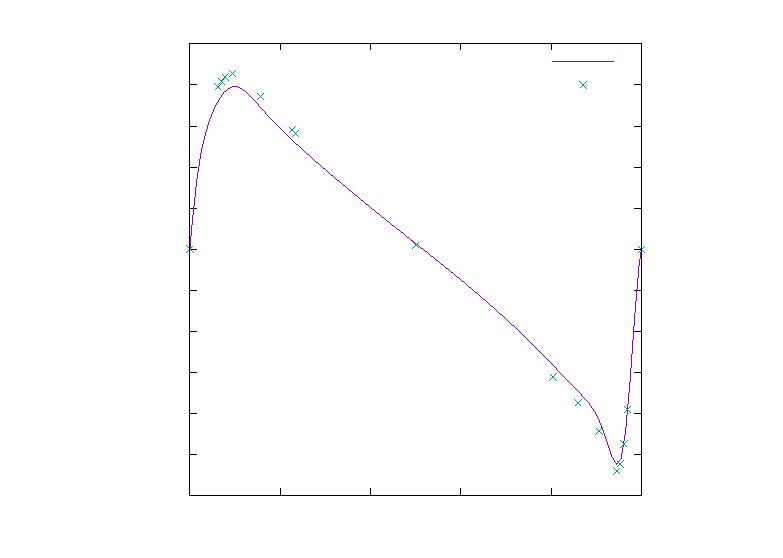
\includegraphics{DrivenCavity/v3200}}%
    \gplfronttext
  \end{picture}%
\endgroup
}
		\caption{$Re=3200$}
	\end{subfigure}%
	\begin{subfigure}{0.5\textwidth}
		\center
		\resizebox{1.4\textwidth}{!}{% GNUPLOT: LaTeX picture with Postscript
\begingroup
  \makeatletter
  \providecommand\color[2][]{%
    \GenericError{(gnuplot) \space\space\space\@spaces}{%
      Package color not loaded in conjunction with
      terminal option `colourtext'%
    }{See the gnuplot documentation for explanation.%
    }{Either use 'blacktext' in gnuplot or load the package
      color.sty in LaTeX.}%
    \renewcommand\color[2][]{}%
  }%
  \providecommand\includegraphics[2][]{%
    \GenericError{(gnuplot) \space\space\space\@spaces}{%
      Package graphicx or graphics not loaded%
    }{See the gnuplot documentation for explanation.%
    }{The gnuplot epslatex terminal needs graphicx.sty or graphics.sty.}%
    \renewcommand\includegraphics[2][]{}%
  }%
  \providecommand\rotatebox[2]{#2}%
  \@ifundefined{ifGPcolor}{%
    \newif\ifGPcolor
    \GPcolortrue
  }{}%
  \@ifundefined{ifGPblacktext}{%
    \newif\ifGPblacktext
    \GPblacktexttrue
  }{}%
  % define a \g@addto@macro without @ in the name:
  \let\gplgaddtomacro\g@addto@macro
  % define empty templates for all commands taking text:
  \gdef\gplbacktext{}%
  \gdef\gplfronttext{}%
  \makeatother
  \ifGPblacktext
    % no textcolor at all
    \def\colorrgb#1{}%
    \def\colorgray#1{}%
  \else
    % gray or color?
    \ifGPcolor
      \def\colorrgb#1{\color[rgb]{#1}}%
      \def\colorgray#1{\color[gray]{#1}}%
      \expandafter\def\csname LTw\endcsname{\color{white}}%
      \expandafter\def\csname LTb\endcsname{\color{black}}%
      \expandafter\def\csname LTa\endcsname{\color{black}}%
      \expandafter\def\csname LT0\endcsname{\color[rgb]{1,0,0}}%
      \expandafter\def\csname LT1\endcsname{\color[rgb]{0,1,0}}%
      \expandafter\def\csname LT2\endcsname{\color[rgb]{0,0,1}}%
      \expandafter\def\csname LT3\endcsname{\color[rgb]{1,0,1}}%
      \expandafter\def\csname LT4\endcsname{\color[rgb]{0,1,1}}%
      \expandafter\def\csname LT5\endcsname{\color[rgb]{1,1,0}}%
      \expandafter\def\csname LT6\endcsname{\color[rgb]{0,0,0}}%
      \expandafter\def\csname LT7\endcsname{\color[rgb]{1,0.3,0}}%
      \expandafter\def\csname LT8\endcsname{\color[rgb]{0.5,0.5,0.5}}%
    \else
      % gray
      \def\colorrgb#1{\color{black}}%
      \def\colorgray#1{\color[gray]{#1}}%
      \expandafter\def\csname LTw\endcsname{\color{white}}%
      \expandafter\def\csname LTb\endcsname{\color{black}}%
      \expandafter\def\csname LTa\endcsname{\color{black}}%
      \expandafter\def\csname LT0\endcsname{\color{black}}%
      \expandafter\def\csname LT1\endcsname{\color{black}}%
      \expandafter\def\csname LT2\endcsname{\color{black}}%
      \expandafter\def\csname LT3\endcsname{\color{black}}%
      \expandafter\def\csname LT4\endcsname{\color{black}}%
      \expandafter\def\csname LT5\endcsname{\color{black}}%
      \expandafter\def\csname LT6\endcsname{\color{black}}%
      \expandafter\def\csname LT7\endcsname{\color{black}}%
      \expandafter\def\csname LT8\endcsname{\color{black}}%
    \fi
  \fi
    \setlength{\unitlength}{0.0500bp}%
    \ifx\gptboxheight\undefined%
      \newlength{\gptboxheight}%
      \newlength{\gptboxwidth}%
      \newsavebox{\gptboxtext}%
    \fi%
    \setlength{\fboxrule}{0.5pt}%
    \setlength{\fboxsep}{1pt}%
\begin{picture}(7200.00,5040.00)%
    \gplgaddtomacro\gplbacktext{%
      \csname LTb\endcsname%
      \put(1531,440){\makebox(0,0)[r]{\strut{}$-0.6$}}%
      \put(1531,834){\makebox(0,0)[r]{\strut{}$-0.5$}}%
      \put(1531,1228){\makebox(0,0)[r]{\strut{}$-0.4$}}%
      \put(1531,1622){\makebox(0,0)[r]{\strut{}$-0.3$}}%
      \put(1531,2016){\makebox(0,0)[r]{\strut{}$-0.2$}}%
      \put(1531,2410){\makebox(0,0)[r]{\strut{}$-0.1$}}%
      \put(1531,2805){\makebox(0,0)[r]{\strut{}$0$}}%
      \put(1531,3199){\makebox(0,0)[r]{\strut{}$0.1$}}%
      \put(1531,3593){\makebox(0,0)[r]{\strut{}$0.2$}}%
      \put(1531,3987){\makebox(0,0)[r]{\strut{}$0.3$}}%
      \put(1531,4381){\makebox(0,0)[r]{\strut{}$0.4$}}%
      \put(1531,4775){\makebox(0,0)[r]{\strut{}$0.5$}}%
      \put(1663,220){\makebox(0,0){\strut{}$0$}}%
      \put(2530,220){\makebox(0,0){\strut{}$0.2$}}%
      \put(3397,220){\makebox(0,0){\strut{}$0.4$}}%
      \put(4264,220){\makebox(0,0){\strut{}$0.6$}}%
      \put(5131,220){\makebox(0,0){\strut{}$0.8$}}%
      \put(5998,220){\makebox(0,0){\strut{}$1$}}%
    }%
    \gplgaddtomacro\gplfronttext{%
      \csname LTb\endcsname%
      \put(5011,4602){\makebox(0,0)[r]{\strut{}Calculated}}%
      \csname LTb\endcsname%
      \put(5011,4382){\makebox(0,0)[r]{\strut{}Reference}}%
    }%
    \gplbacktext
    \put(0,0){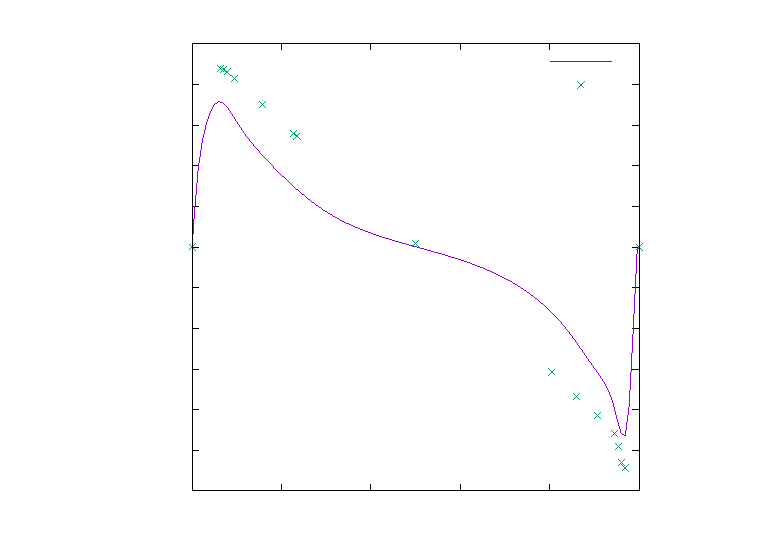
\includegraphics{DrivenCavity/v10000}}%
    \gplfronttext
  \end{picture}%
\endgroup
}
		\caption{$Re=10000$}
	\end{subfigure}
	\caption[Comparison between the reference solution and the calculated one of the vertical velocity along the horizontal line in the geometric center of the cavity]{Comparison between the reference solution and the calculated one of the vertical velocity along the horizontal line in the geometric centre of the cavity \cite{Ghia1982}}
	\label{Drivenvertical}
\end{figure}

As for the distribution of velocities, it can be seen that as the Reynolds increases the variation becomes sharper, especially near the walls, where the gradient of velocities is higher. For the horizontal velocities, the shape of the curve is very different for lower and higher Reynolds.

\begin{figure}[h]
	\centering
	\begin{subfigure}{0.5\textwidth}
		\resizebox{1.4\textwidth}{!}{% GNUPLOT: LaTeX picture with Postscript
\begingroup
  \makeatletter
  \providecommand\color[2][]{%
    \GenericError{(gnuplot) \space\space\space\@spaces}{%
      Package color not loaded in conjunction with
      terminal option `colourtext'%
    }{See the gnuplot documentation for explanation.%
    }{Either use 'blacktext' in gnuplot or load the package
      color.sty in LaTeX.}%
    \renewcommand\color[2][]{}%
  }%
  \providecommand\includegraphics[2][]{%
    \GenericError{(gnuplot) \space\space\space\@spaces}{%
      Package graphicx or graphics not loaded%
    }{See the gnuplot documentation for explanation.%
    }{The gnuplot epslatex terminal needs graphicx.sty or graphics.sty.}%
    \renewcommand\includegraphics[2][]{}%
  }%
  \providecommand\rotatebox[2]{#2}%
  \@ifundefined{ifGPcolor}{%
    \newif\ifGPcolor
    \GPcolortrue
  }{}%
  \@ifundefined{ifGPblacktext}{%
    \newif\ifGPblacktext
    \GPblacktexttrue
  }{}%
  % define a \g@addto@macro without @ in the name:
  \let\gplgaddtomacro\g@addto@macro
  % define empty templates for all commands taking text:
  \gdef\gplbacktext{}%
  \gdef\gplfronttext{}%
  \makeatother
  \ifGPblacktext
    % no textcolor at all
    \def\colorrgb#1{}%
    \def\colorgray#1{}%
  \else
    % gray or color?
    \ifGPcolor
      \def\colorrgb#1{\color[rgb]{#1}}%
      \def\colorgray#1{\color[gray]{#1}}%
      \expandafter\def\csname LTw\endcsname{\color{white}}%
      \expandafter\def\csname LTb\endcsname{\color{black}}%
      \expandafter\def\csname LTa\endcsname{\color{black}}%
      \expandafter\def\csname LT0\endcsname{\color[rgb]{1,0,0}}%
      \expandafter\def\csname LT1\endcsname{\color[rgb]{0,1,0}}%
      \expandafter\def\csname LT2\endcsname{\color[rgb]{0,0,1}}%
      \expandafter\def\csname LT3\endcsname{\color[rgb]{1,0,1}}%
      \expandafter\def\csname LT4\endcsname{\color[rgb]{0,1,1}}%
      \expandafter\def\csname LT5\endcsname{\color[rgb]{1,1,0}}%
      \expandafter\def\csname LT6\endcsname{\color[rgb]{0,0,0}}%
      \expandafter\def\csname LT7\endcsname{\color[rgb]{1,0.3,0}}%
      \expandafter\def\csname LT8\endcsname{\color[rgb]{0.5,0.5,0.5}}%
    \else
      % gray
      \def\colorrgb#1{\color{black}}%
      \def\colorgray#1{\color[gray]{#1}}%
      \expandafter\def\csname LTw\endcsname{\color{white}}%
      \expandafter\def\csname LTb\endcsname{\color{black}}%
      \expandafter\def\csname LTa\endcsname{\color{black}}%
      \expandafter\def\csname LT0\endcsname{\color{black}}%
      \expandafter\def\csname LT1\endcsname{\color{black}}%
      \expandafter\def\csname LT2\endcsname{\color{black}}%
      \expandafter\def\csname LT3\endcsname{\color{black}}%
      \expandafter\def\csname LT4\endcsname{\color{black}}%
      \expandafter\def\csname LT5\endcsname{\color{black}}%
      \expandafter\def\csname LT6\endcsname{\color{black}}%
      \expandafter\def\csname LT7\endcsname{\color{black}}%
      \expandafter\def\csname LT8\endcsname{\color{black}}%
    \fi
  \fi
    \setlength{\unitlength}{0.0500bp}%
    \ifx\gptboxheight\undefined%
      \newlength{\gptboxheight}%
      \newlength{\gptboxwidth}%
      \newsavebox{\gptboxtext}%
    \fi%
    \setlength{\fboxrule}{0.5pt}%
    \setlength{\fboxsep}{1pt}%
\begin{picture}(7200.00,5040.00)%
    \gplgaddtomacro\gplbacktext{%
    }%
    \gplgaddtomacro\gplfronttext{%
      \csname LTb\endcsname%
      \put(1908,624){\makebox(0,0){\strut{}$0$}}%
      \put(2585,624){\makebox(0,0){\strut{}$0.2$}}%
      \put(3262,624){\makebox(0,0){\strut{}$0.4$}}%
      \put(3938,624){\makebox(0,0){\strut{}$0.6$}}%
      \put(4615,624){\makebox(0,0){\strut{}$0.8$}}%
      \put(5292,624){\makebox(0,0){\strut{}$1$}}%
      \put(1720,938){\makebox(0,0)[r]{\strut{}$0$}}%
      \put(1720,1615){\makebox(0,0)[r]{\strut{}$0.2$}}%
      \put(1720,2292){\makebox(0,0)[r]{\strut{}$0.4$}}%
      \put(1720,2968){\makebox(0,0)[r]{\strut{}$0.6$}}%
      \put(1720,3645){\makebox(0,0)[r]{\strut{}$0.8$}}%
      \put(1720,4322){\makebox(0,0)[r]{\strut{}$1$}}%
      \put(5678,938){\makebox(0,0)[l]{\strut{}$-0.4$}}%
      \put(5678,1421){\makebox(0,0)[l]{\strut{}$-0.2$}}%
      \put(5678,1904){\makebox(0,0)[l]{\strut{}$0$}}%
      \put(5678,2388){\makebox(0,0)[l]{\strut{}$0.2$}}%
      \put(5678,2871){\makebox(0,0)[l]{\strut{}$0.4$}}%
      \put(5678,3355){\makebox(0,0)[l]{\strut{}$0.6$}}%
      \put(5678,3838){\makebox(0,0)[l]{\strut{}$0.8$}}%
      \put(5678,4322){\makebox(0,0)[l]{\strut{}$1$}}%
    }%
    \gplbacktext
    \put(0,0){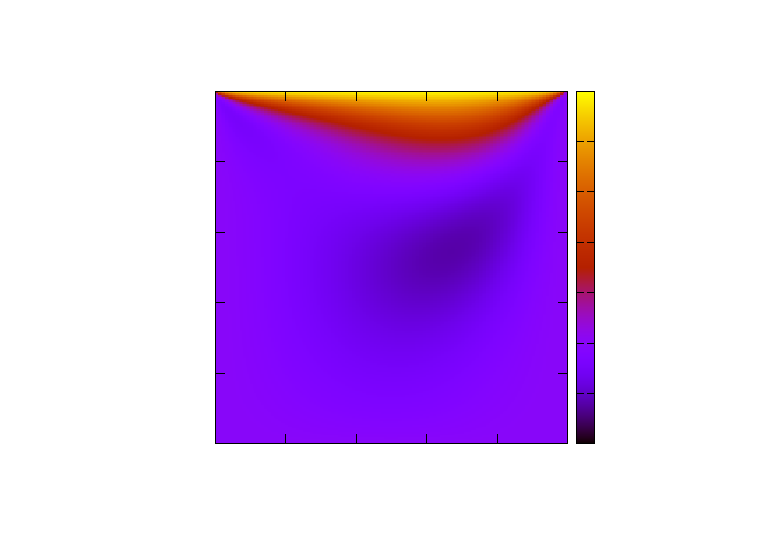
\includegraphics{Ru100}}%
    \gplfronttext
  \end{picture}%
\endgroup
}
		\caption{$Re=100$}
	\end{subfigure}%
	\begin{subfigure}{0.5\textwidth}
		\resizebox{1.4\textwidth}{!}{% GNUPLOT: LaTeX picture with Postscript
\begingroup
  \makeatletter
  \providecommand\color[2][]{%
    \GenericError{(gnuplot) \space\space\space\@spaces}{%
      Package color not loaded in conjunction with
      terminal option `colourtext'%
    }{See the gnuplot documentation for explanation.%
    }{Either use 'blacktext' in gnuplot or load the package
      color.sty in LaTeX.}%
    \renewcommand\color[2][]{}%
  }%
  \providecommand\includegraphics[2][]{%
    \GenericError{(gnuplot) \space\space\space\@spaces}{%
      Package graphicx or graphics not loaded%
    }{See the gnuplot documentation for explanation.%
    }{The gnuplot epslatex terminal needs graphicx.sty or graphics.sty.}%
    \renewcommand\includegraphics[2][]{}%
  }%
  \providecommand\rotatebox[2]{#2}%
  \@ifundefined{ifGPcolor}{%
    \newif\ifGPcolor
    \GPcolortrue
  }{}%
  \@ifundefined{ifGPblacktext}{%
    \newif\ifGPblacktext
    \GPblacktexttrue
  }{}%
  % define a \g@addto@macro without @ in the name:
  \let\gplgaddtomacro\g@addto@macro
  % define empty templates for all commands taking text:
  \gdef\gplbacktext{}%
  \gdef\gplfronttext{}%
  \makeatother
  \ifGPblacktext
    % no textcolor at all
    \def\colorrgb#1{}%
    \def\colorgray#1{}%
  \else
    % gray or color?
    \ifGPcolor
      \def\colorrgb#1{\color[rgb]{#1}}%
      \def\colorgray#1{\color[gray]{#1}}%
      \expandafter\def\csname LTw\endcsname{\color{white}}%
      \expandafter\def\csname LTb\endcsname{\color{black}}%
      \expandafter\def\csname LTa\endcsname{\color{black}}%
      \expandafter\def\csname LT0\endcsname{\color[rgb]{1,0,0}}%
      \expandafter\def\csname LT1\endcsname{\color[rgb]{0,1,0}}%
      \expandafter\def\csname LT2\endcsname{\color[rgb]{0,0,1}}%
      \expandafter\def\csname LT3\endcsname{\color[rgb]{1,0,1}}%
      \expandafter\def\csname LT4\endcsname{\color[rgb]{0,1,1}}%
      \expandafter\def\csname LT5\endcsname{\color[rgb]{1,1,0}}%
      \expandafter\def\csname LT6\endcsname{\color[rgb]{0,0,0}}%
      \expandafter\def\csname LT7\endcsname{\color[rgb]{1,0.3,0}}%
      \expandafter\def\csname LT8\endcsname{\color[rgb]{0.5,0.5,0.5}}%
    \else
      % gray
      \def\colorrgb#1{\color{black}}%
      \def\colorgray#1{\color[gray]{#1}}%
      \expandafter\def\csname LTw\endcsname{\color{white}}%
      \expandafter\def\csname LTb\endcsname{\color{black}}%
      \expandafter\def\csname LTa\endcsname{\color{black}}%
      \expandafter\def\csname LT0\endcsname{\color{black}}%
      \expandafter\def\csname LT1\endcsname{\color{black}}%
      \expandafter\def\csname LT2\endcsname{\color{black}}%
      \expandafter\def\csname LT3\endcsname{\color{black}}%
      \expandafter\def\csname LT4\endcsname{\color{black}}%
      \expandafter\def\csname LT5\endcsname{\color{black}}%
      \expandafter\def\csname LT6\endcsname{\color{black}}%
      \expandafter\def\csname LT7\endcsname{\color{black}}%
      \expandafter\def\csname LT8\endcsname{\color{black}}%
    \fi
  \fi
    \setlength{\unitlength}{0.0500bp}%
    \ifx\gptboxheight\undefined%
      \newlength{\gptboxheight}%
      \newlength{\gptboxwidth}%
      \newsavebox{\gptboxtext}%
    \fi%
    \setlength{\fboxrule}{0.5pt}%
    \setlength{\fboxsep}{1pt}%
\begin{picture}(7200.00,5040.00)%
    \gplgaddtomacro\gplbacktext{%
    }%
    \gplgaddtomacro\gplfronttext{%
      \csname LTb\endcsname%
      \put(1908,624){\makebox(0,0){\strut{}$0$}}%
      \put(2585,624){\makebox(0,0){\strut{}$0.2$}}%
      \put(3262,624){\makebox(0,0){\strut{}$0.4$}}%
      \put(3938,624){\makebox(0,0){\strut{}$0.6$}}%
      \put(4615,624){\makebox(0,0){\strut{}$0.8$}}%
      \put(5292,624){\makebox(0,0){\strut{}$1$}}%
      \put(1720,938){\makebox(0,0)[r]{\strut{}$0$}}%
      \put(1720,1615){\makebox(0,0)[r]{\strut{}$0.2$}}%
      \put(1720,2292){\makebox(0,0)[r]{\strut{}$0.4$}}%
      \put(1720,2968){\makebox(0,0)[r]{\strut{}$0.6$}}%
      \put(1720,3645){\makebox(0,0)[r]{\strut{}$0.8$}}%
      \put(1720,4322){\makebox(0,0)[r]{\strut{}$1$}}%
      \put(5678,938){\makebox(0,0)[l]{\strut{}$-0.4$}}%
      \put(5678,1421){\makebox(0,0)[l]{\strut{}$-0.2$}}%
      \put(5678,1904){\makebox(0,0)[l]{\strut{}$0$}}%
      \put(5678,2388){\makebox(0,0)[l]{\strut{}$0.2$}}%
      \put(5678,2871){\makebox(0,0)[l]{\strut{}$0.4$}}%
      \put(5678,3355){\makebox(0,0)[l]{\strut{}$0.6$}}%
      \put(5678,3838){\makebox(0,0)[l]{\strut{}$0.8$}}%
      \put(5678,4322){\makebox(0,0)[l]{\strut{}$1$}}%
    }%
    \gplbacktext
    \put(0,0){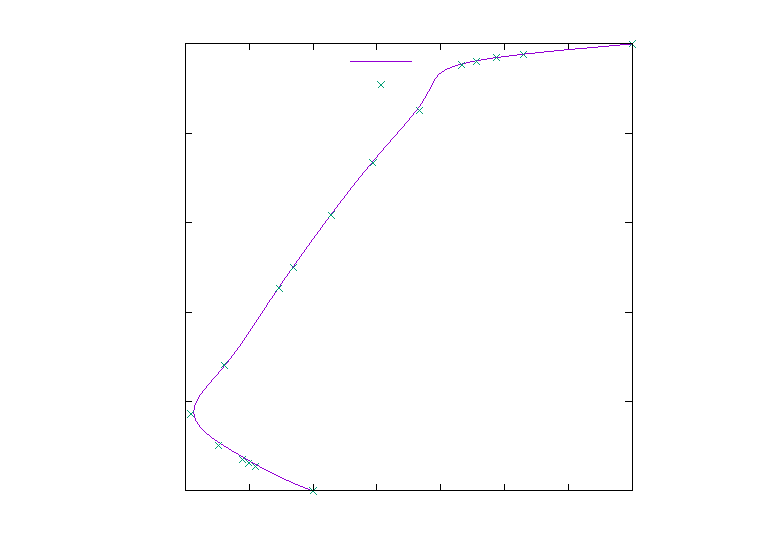
\includegraphics{u1000}}%
    \gplfronttext
  \end{picture}%
\endgroup
}
		\caption{$Re=1000$}
	\end{subfigure}
	\begin{subfigure}{0.5\textwidth}
		\resizebox{1.4\textwidth}{!}{% GNUPLOT: LaTeX picture with Postscript
\begingroup
  \makeatletter
  \providecommand\color[2][]{%
    \GenericError{(gnuplot) \space\space\space\@spaces}{%
      Package color not loaded in conjunction with
      terminal option `colourtext'%
    }{See the gnuplot documentation for explanation.%
    }{Either use 'blacktext' in gnuplot or load the package
      color.sty in LaTeX.}%
    \renewcommand\color[2][]{}%
  }%
  \providecommand\includegraphics[2][]{%
    \GenericError{(gnuplot) \space\space\space\@spaces}{%
      Package graphicx or graphics not loaded%
    }{See the gnuplot documentation for explanation.%
    }{The gnuplot epslatex terminal needs graphicx.sty or graphics.sty.}%
    \renewcommand\includegraphics[2][]{}%
  }%
  \providecommand\rotatebox[2]{#2}%
  \@ifundefined{ifGPcolor}{%
    \newif\ifGPcolor
    \GPcolortrue
  }{}%
  \@ifundefined{ifGPblacktext}{%
    \newif\ifGPblacktext
    \GPblacktexttrue
  }{}%
  % define a \g@addto@macro without @ in the name:
  \let\gplgaddtomacro\g@addto@macro
  % define empty templates for all commands taking text:
  \gdef\gplbacktext{}%
  \gdef\gplfronttext{}%
  \makeatother
  \ifGPblacktext
    % no textcolor at all
    \def\colorrgb#1{}%
    \def\colorgray#1{}%
  \else
    % gray or color?
    \ifGPcolor
      \def\colorrgb#1{\color[rgb]{#1}}%
      \def\colorgray#1{\color[gray]{#1}}%
      \expandafter\def\csname LTw\endcsname{\color{white}}%
      \expandafter\def\csname LTb\endcsname{\color{black}}%
      \expandafter\def\csname LTa\endcsname{\color{black}}%
      \expandafter\def\csname LT0\endcsname{\color[rgb]{1,0,0}}%
      \expandafter\def\csname LT1\endcsname{\color[rgb]{0,1,0}}%
      \expandafter\def\csname LT2\endcsname{\color[rgb]{0,0,1}}%
      \expandafter\def\csname LT3\endcsname{\color[rgb]{1,0,1}}%
      \expandafter\def\csname LT4\endcsname{\color[rgb]{0,1,1}}%
      \expandafter\def\csname LT5\endcsname{\color[rgb]{1,1,0}}%
      \expandafter\def\csname LT6\endcsname{\color[rgb]{0,0,0}}%
      \expandafter\def\csname LT7\endcsname{\color[rgb]{1,0.3,0}}%
      \expandafter\def\csname LT8\endcsname{\color[rgb]{0.5,0.5,0.5}}%
    \else
      % gray
      \def\colorrgb#1{\color{black}}%
      \def\colorgray#1{\color[gray]{#1}}%
      \expandafter\def\csname LTw\endcsname{\color{white}}%
      \expandafter\def\csname LTb\endcsname{\color{black}}%
      \expandafter\def\csname LTa\endcsname{\color{black}}%
      \expandafter\def\csname LT0\endcsname{\color{black}}%
      \expandafter\def\csname LT1\endcsname{\color{black}}%
      \expandafter\def\csname LT2\endcsname{\color{black}}%
      \expandafter\def\csname LT3\endcsname{\color{black}}%
      \expandafter\def\csname LT4\endcsname{\color{black}}%
      \expandafter\def\csname LT5\endcsname{\color{black}}%
      \expandafter\def\csname LT6\endcsname{\color{black}}%
      \expandafter\def\csname LT7\endcsname{\color{black}}%
      \expandafter\def\csname LT8\endcsname{\color{black}}%
    \fi
  \fi
    \setlength{\unitlength}{0.0500bp}%
    \ifx\gptboxheight\undefined%
      \newlength{\gptboxheight}%
      \newlength{\gptboxwidth}%
      \newsavebox{\gptboxtext}%
    \fi%
    \setlength{\fboxrule}{0.5pt}%
    \setlength{\fboxsep}{1pt}%
\begin{picture}(7200.00,5040.00)%
    \gplgaddtomacro\gplbacktext{%
    }%
    \gplgaddtomacro\gplfronttext{%
      \csname LTb\endcsname%
      \put(1908,624){\makebox(0,0){\strut{}$0$}}%
      \put(2585,624){\makebox(0,0){\strut{}$0.2$}}%
      \put(3262,624){\makebox(0,0){\strut{}$0.4$}}%
      \put(3938,624){\makebox(0,0){\strut{}$0.6$}}%
      \put(4615,624){\makebox(0,0){\strut{}$0.8$}}%
      \put(5292,624){\makebox(0,0){\strut{}$1$}}%
      \put(1720,938){\makebox(0,0)[r]{\strut{}$0$}}%
      \put(1720,1615){\makebox(0,0)[r]{\strut{}$0.2$}}%
      \put(1720,2292){\makebox(0,0)[r]{\strut{}$0.4$}}%
      \put(1720,2968){\makebox(0,0)[r]{\strut{}$0.6$}}%
      \put(1720,3645){\makebox(0,0)[r]{\strut{}$0.8$}}%
      \put(1720,4322){\makebox(0,0)[r]{\strut{}$1$}}%
      \put(5678,938){\makebox(0,0)[l]{\strut{}$-0.4$}}%
      \put(5678,1421){\makebox(0,0)[l]{\strut{}$-0.2$}}%
      \put(5678,1904){\makebox(0,0)[l]{\strut{}$0$}}%
      \put(5678,2388){\makebox(0,0)[l]{\strut{}$0.2$}}%
      \put(5678,2871){\makebox(0,0)[l]{\strut{}$0.4$}}%
      \put(5678,3355){\makebox(0,0)[l]{\strut{}$0.6$}}%
      \put(5678,3838){\makebox(0,0)[l]{\strut{}$0.8$}}%
      \put(5678,4322){\makebox(0,0)[l]{\strut{}$1$}}%
    }%
    \gplbacktext
    \put(0,0){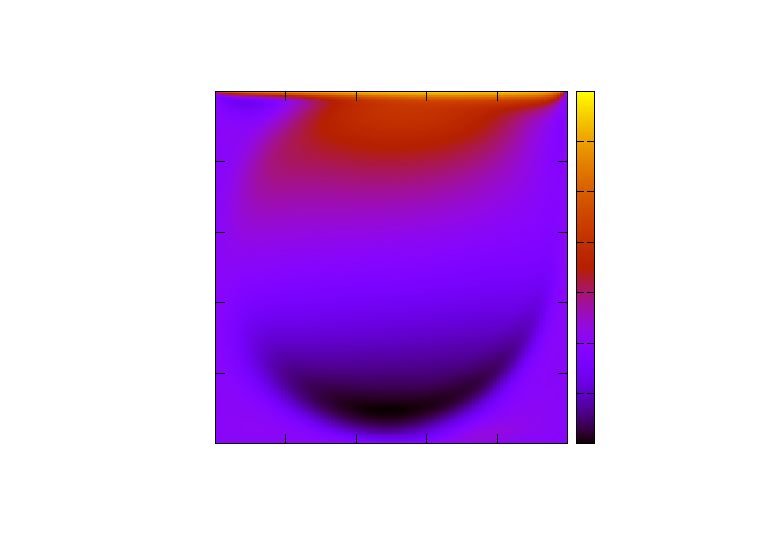
\includegraphics{Ru3200}}%
    \gplfronttext
  \end{picture}%
\endgroup
}
		\caption{$Re=3200$}
	\end{subfigure}%
	\begin{subfigure}{0.5\textwidth}
		\center
		\resizebox{1.4\textwidth}{!}{% GNUPLOT: LaTeX picture with Postscript
\begingroup
  \makeatletter
  \providecommand\color[2][]{%
    \GenericError{(gnuplot) \space\space\space\@spaces}{%
      Package color not loaded in conjunction with
      terminal option `colourtext'%
    }{See the gnuplot documentation for explanation.%
    }{Either use 'blacktext' in gnuplot or load the package
      color.sty in LaTeX.}%
    \renewcommand\color[2][]{}%
  }%
  \providecommand\includegraphics[2][]{%
    \GenericError{(gnuplot) \space\space\space\@spaces}{%
      Package graphicx or graphics not loaded%
    }{See the gnuplot documentation for explanation.%
    }{The gnuplot epslatex terminal needs graphicx.sty or graphics.sty.}%
    \renewcommand\includegraphics[2][]{}%
  }%
  \providecommand\rotatebox[2]{#2}%
  \@ifundefined{ifGPcolor}{%
    \newif\ifGPcolor
    \GPcolortrue
  }{}%
  \@ifundefined{ifGPblacktext}{%
    \newif\ifGPblacktext
    \GPblacktexttrue
  }{}%
  % define a \g@addto@macro without @ in the name:
  \let\gplgaddtomacro\g@addto@macro
  % define empty templates for all commands taking text:
  \gdef\gplbacktext{}%
  \gdef\gplfronttext{}%
  \makeatother
  \ifGPblacktext
    % no textcolor at all
    \def\colorrgb#1{}%
    \def\colorgray#1{}%
  \else
    % gray or color?
    \ifGPcolor
      \def\colorrgb#1{\color[rgb]{#1}}%
      \def\colorgray#1{\color[gray]{#1}}%
      \expandafter\def\csname LTw\endcsname{\color{white}}%
      \expandafter\def\csname LTb\endcsname{\color{black}}%
      \expandafter\def\csname LTa\endcsname{\color{black}}%
      \expandafter\def\csname LT0\endcsname{\color[rgb]{1,0,0}}%
      \expandafter\def\csname LT1\endcsname{\color[rgb]{0,1,0}}%
      \expandafter\def\csname LT2\endcsname{\color[rgb]{0,0,1}}%
      \expandafter\def\csname LT3\endcsname{\color[rgb]{1,0,1}}%
      \expandafter\def\csname LT4\endcsname{\color[rgb]{0,1,1}}%
      \expandafter\def\csname LT5\endcsname{\color[rgb]{1,1,0}}%
      \expandafter\def\csname LT6\endcsname{\color[rgb]{0,0,0}}%
      \expandafter\def\csname LT7\endcsname{\color[rgb]{1,0.3,0}}%
      \expandafter\def\csname LT8\endcsname{\color[rgb]{0.5,0.5,0.5}}%
    \else
      % gray
      \def\colorrgb#1{\color{black}}%
      \def\colorgray#1{\color[gray]{#1}}%
      \expandafter\def\csname LTw\endcsname{\color{white}}%
      \expandafter\def\csname LTb\endcsname{\color{black}}%
      \expandafter\def\csname LTa\endcsname{\color{black}}%
      \expandafter\def\csname LT0\endcsname{\color{black}}%
      \expandafter\def\csname LT1\endcsname{\color{black}}%
      \expandafter\def\csname LT2\endcsname{\color{black}}%
      \expandafter\def\csname LT3\endcsname{\color{black}}%
      \expandafter\def\csname LT4\endcsname{\color{black}}%
      \expandafter\def\csname LT5\endcsname{\color{black}}%
      \expandafter\def\csname LT6\endcsname{\color{black}}%
      \expandafter\def\csname LT7\endcsname{\color{black}}%
      \expandafter\def\csname LT8\endcsname{\color{black}}%
    \fi
  \fi
    \setlength{\unitlength}{0.0500bp}%
    \ifx\gptboxheight\undefined%
      \newlength{\gptboxheight}%
      \newlength{\gptboxwidth}%
      \newsavebox{\gptboxtext}%
    \fi%
    \setlength{\fboxrule}{0.5pt}%
    \setlength{\fboxsep}{1pt}%
\begin{picture}(7200.00,5040.00)%
    \gplgaddtomacro\gplbacktext{%
    }%
    \gplgaddtomacro\gplfronttext{%
      \put(1908,624){\makebox(0,0){\strut{}$0$}}%
      \put(2585,624){\makebox(0,0){\strut{}$0.2$}}%
      \put(3262,624){\makebox(0,0){\strut{}$0.4$}}%
      \put(3938,624){\makebox(0,0){\strut{}$0.6$}}%
      \put(4615,624){\makebox(0,0){\strut{}$0.8$}}%
      \put(5292,624){\makebox(0,0){\strut{}$1$}}%
      \put(1720,938){\makebox(0,0)[r]{\strut{}$0$}}%
      \put(1720,1615){\makebox(0,0)[r]{\strut{}$0.2$}}%
      \put(1720,2292){\makebox(0,0)[r]{\strut{}$0.4$}}%
      \put(1720,2968){\makebox(0,0)[r]{\strut{}$0.6$}}%
      \put(1720,3645){\makebox(0,0)[r]{\strut{}$0.8$}}%
      \put(1720,4322){\makebox(0,0)[r]{\strut{}$1$}}%
      \put(5678,938){\makebox(0,0)[l]{\strut{}$-0.4$}}%
      \put(5678,1421){\makebox(0,0)[l]{\strut{}$-0.2$}}%
      \put(5678,1904){\makebox(0,0)[l]{\strut{}$0$}}%
      \put(5678,2388){\makebox(0,0)[l]{\strut{}$0.2$}}%
      \put(5678,2871){\makebox(0,0)[l]{\strut{}$0.4$}}%
      \put(5678,3355){\makebox(0,0)[l]{\strut{}$0.6$}}%
      \put(5678,3838){\makebox(0,0)[l]{\strut{}$0.8$}}%
      \put(5678,4322){\makebox(0,0)[l]{\strut{}$1$}}%
    }%
    \gplbacktext
    \put(0,0){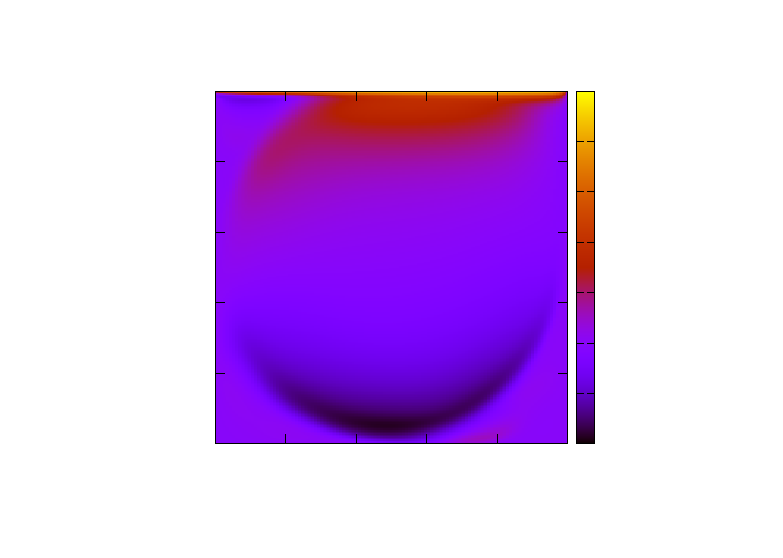
\includegraphics{DrivenCavity/Ru10000}}%
    \gplfronttext
  \end{picture}%
\endgroup
}
		\caption{$Re=10000$}
	\end{subfigure}
	\caption{Horizontal velocity in the cavity}
	\label{DrivenHorizontalDomain}
\end{figure}

Looking at the variation of the horizontal velocity in the whole domain (figure \ref{DrivenHorizontalDomain}), for lower Reynolds, there is only a small movement in the top of the cavity. But as the Re increases, more fluid becomes involved with the clockwise rotation, increasing its radius. For $Re=10000$, the distribution shows that only the outer radius of the cavity rotates. However, these results may not be realistic due to the error obtained at high Reynolds.

\begin{figure}[h]
	\centering
	\begin{subfigure}{0.5\textwidth}
		\resizebox{1.4\textwidth}{!}{% GNUPLOT: LaTeX picture with Postscript
\begingroup
  \makeatletter
  \providecommand\color[2][]{%
    \GenericError{(gnuplot) \space\space\space\@spaces}{%
      Package color not loaded in conjunction with
      terminal option `colourtext'%
    }{See the gnuplot documentation for explanation.%
    }{Either use 'blacktext' in gnuplot or load the package
      color.sty in LaTeX.}%
    \renewcommand\color[2][]{}%
  }%
  \providecommand\includegraphics[2][]{%
    \GenericError{(gnuplot) \space\space\space\@spaces}{%
      Package graphicx or graphics not loaded%
    }{See the gnuplot documentation for explanation.%
    }{The gnuplot epslatex terminal needs graphicx.sty or graphics.sty.}%
    \renewcommand\includegraphics[2][]{}%
  }%
  \providecommand\rotatebox[2]{#2}%
  \@ifundefined{ifGPcolor}{%
    \newif\ifGPcolor
    \GPcolortrue
  }{}%
  \@ifundefined{ifGPblacktext}{%
    \newif\ifGPblacktext
    \GPblacktexttrue
  }{}%
  % define a \g@addto@macro without @ in the name:
  \let\gplgaddtomacro\g@addto@macro
  % define empty templates for all commands taking text:
  \gdef\gplbacktext{}%
  \gdef\gplfronttext{}%
  \makeatother
  \ifGPblacktext
    % no textcolor at all
    \def\colorrgb#1{}%
    \def\colorgray#1{}%
  \else
    % gray or color?
    \ifGPcolor
      \def\colorrgb#1{\color[rgb]{#1}}%
      \def\colorgray#1{\color[gray]{#1}}%
      \expandafter\def\csname LTw\endcsname{\color{white}}%
      \expandafter\def\csname LTb\endcsname{\color{black}}%
      \expandafter\def\csname LTa\endcsname{\color{black}}%
      \expandafter\def\csname LT0\endcsname{\color[rgb]{1,0,0}}%
      \expandafter\def\csname LT1\endcsname{\color[rgb]{0,1,0}}%
      \expandafter\def\csname LT2\endcsname{\color[rgb]{0,0,1}}%
      \expandafter\def\csname LT3\endcsname{\color[rgb]{1,0,1}}%
      \expandafter\def\csname LT4\endcsname{\color[rgb]{0,1,1}}%
      \expandafter\def\csname LT5\endcsname{\color[rgb]{1,1,0}}%
      \expandafter\def\csname LT6\endcsname{\color[rgb]{0,0,0}}%
      \expandafter\def\csname LT7\endcsname{\color[rgb]{1,0.3,0}}%
      \expandafter\def\csname LT8\endcsname{\color[rgb]{0.5,0.5,0.5}}%
    \else
      % gray
      \def\colorrgb#1{\color{black}}%
      \def\colorgray#1{\color[gray]{#1}}%
      \expandafter\def\csname LTw\endcsname{\color{white}}%
      \expandafter\def\csname LTb\endcsname{\color{black}}%
      \expandafter\def\csname LTa\endcsname{\color{black}}%
      \expandafter\def\csname LT0\endcsname{\color{black}}%
      \expandafter\def\csname LT1\endcsname{\color{black}}%
      \expandafter\def\csname LT2\endcsname{\color{black}}%
      \expandafter\def\csname LT3\endcsname{\color{black}}%
      \expandafter\def\csname LT4\endcsname{\color{black}}%
      \expandafter\def\csname LT5\endcsname{\color{black}}%
      \expandafter\def\csname LT6\endcsname{\color{black}}%
      \expandafter\def\csname LT7\endcsname{\color{black}}%
      \expandafter\def\csname LT8\endcsname{\color{black}}%
    \fi
  \fi
    \setlength{\unitlength}{0.0500bp}%
    \ifx\gptboxheight\undefined%
      \newlength{\gptboxheight}%
      \newlength{\gptboxwidth}%
      \newsavebox{\gptboxtext}%
    \fi%
    \setlength{\fboxrule}{0.5pt}%
    \setlength{\fboxsep}{1pt}%
\begin{picture}(7200.00,5040.00)%
    \gplgaddtomacro\gplbacktext{%
    }%
    \gplgaddtomacro\gplfronttext{%
      \put(1908,624){\makebox(0,0){\strut{}$0$}}%
      \put(2585,624){\makebox(0,0){\strut{}$0.2$}}%
      \put(3262,624){\makebox(0,0){\strut{}$0.4$}}%
      \put(3938,624){\makebox(0,0){\strut{}$0.6$}}%
      \put(4615,624){\makebox(0,0){\strut{}$0.8$}}%
      \put(5292,624){\makebox(0,0){\strut{}$1$}}%
      \put(1720,938){\makebox(0,0)[r]{\strut{}$0$}}%
      \put(1720,1615){\makebox(0,0)[r]{\strut{}$0.2$}}%
      \put(1720,2292){\makebox(0,0)[r]{\strut{}$0.4$}}%
      \put(1720,2968){\makebox(0,0)[r]{\strut{}$0.6$}}%
      \put(1720,3645){\makebox(0,0)[r]{\strut{}$0.8$}}%
      \put(1720,4322){\makebox(0,0)[r]{\strut{}$1$}}%
      \put(5678,938){\makebox(0,0)[l]{\strut{}$-0.6$}}%
      \put(5678,1276){\makebox(0,0)[l]{\strut{}$-0.5$}}%
      \put(5678,1614){\makebox(0,0)[l]{\strut{}$-0.4$}}%
      \put(5678,1953){\makebox(0,0)[l]{\strut{}$-0.3$}}%
      \put(5678,2291){\makebox(0,0)[l]{\strut{}$-0.2$}}%
      \put(5678,2630){\makebox(0,0)[l]{\strut{}$-0.1$}}%
      \put(5678,2968){\makebox(0,0)[l]{\strut{}$0$}}%
      \put(5678,3306){\makebox(0,0)[l]{\strut{}$0.1$}}%
      \put(5678,3645){\makebox(0,0)[l]{\strut{}$0.2$}}%
      \put(5678,3983){\makebox(0,0)[l]{\strut{}$0.3$}}%
      \put(5678,4322){\makebox(0,0)[l]{\strut{}$0.4$}}%
    }%
    \gplbacktext
    \put(0,0){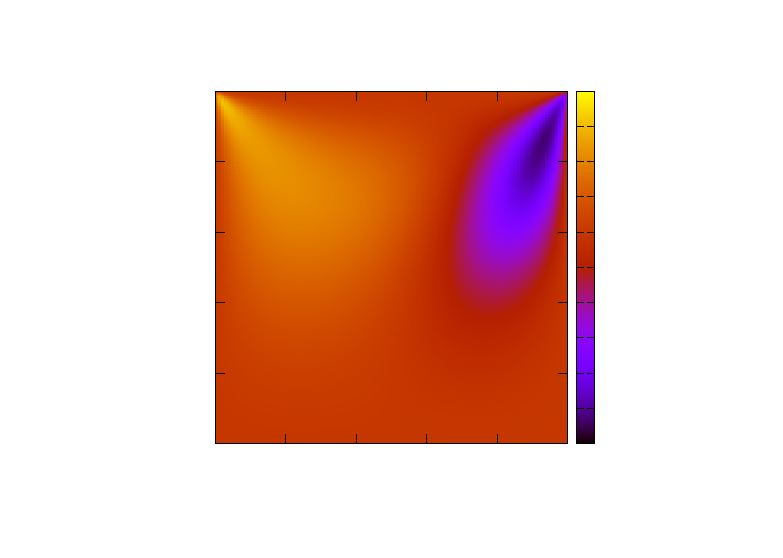
\includegraphics{DrivenCavity/Rv100}}%
    \gplfronttext
  \end{picture}%
\endgroup
}
		\caption{$Re=100$}
	\end{subfigure}%
	\begin{subfigure}{0.5\textwidth}
		\resizebox{1.4\textwidth}{!}{% GNUPLOT: LaTeX picture with Postscript
\begingroup
  \makeatletter
  \providecommand\color[2][]{%
    \GenericError{(gnuplot) \space\space\space\@spaces}{%
      Package color not loaded in conjunction with
      terminal option `colourtext'%
    }{See the gnuplot documentation for explanation.%
    }{Either use 'blacktext' in gnuplot or load the package
      color.sty in LaTeX.}%
    \renewcommand\color[2][]{}%
  }%
  \providecommand\includegraphics[2][]{%
    \GenericError{(gnuplot) \space\space\space\@spaces}{%
      Package graphicx or graphics not loaded%
    }{See the gnuplot documentation for explanation.%
    }{The gnuplot epslatex terminal needs graphicx.sty or graphics.sty.}%
    \renewcommand\includegraphics[2][]{}%
  }%
  \providecommand\rotatebox[2]{#2}%
  \@ifundefined{ifGPcolor}{%
    \newif\ifGPcolor
    \GPcolortrue
  }{}%
  \@ifundefined{ifGPblacktext}{%
    \newif\ifGPblacktext
    \GPblacktexttrue
  }{}%
  % define a \g@addto@macro without @ in the name:
  \let\gplgaddtomacro\g@addto@macro
  % define empty templates for all commands taking text:
  \gdef\gplbacktext{}%
  \gdef\gplfronttext{}%
  \makeatother
  \ifGPblacktext
    % no textcolor at all
    \def\colorrgb#1{}%
    \def\colorgray#1{}%
  \else
    % gray or color?
    \ifGPcolor
      \def\colorrgb#1{\color[rgb]{#1}}%
      \def\colorgray#1{\color[gray]{#1}}%
      \expandafter\def\csname LTw\endcsname{\color{white}}%
      \expandafter\def\csname LTb\endcsname{\color{black}}%
      \expandafter\def\csname LTa\endcsname{\color{black}}%
      \expandafter\def\csname LT0\endcsname{\color[rgb]{1,0,0}}%
      \expandafter\def\csname LT1\endcsname{\color[rgb]{0,1,0}}%
      \expandafter\def\csname LT2\endcsname{\color[rgb]{0,0,1}}%
      \expandafter\def\csname LT3\endcsname{\color[rgb]{1,0,1}}%
      \expandafter\def\csname LT4\endcsname{\color[rgb]{0,1,1}}%
      \expandafter\def\csname LT5\endcsname{\color[rgb]{1,1,0}}%
      \expandafter\def\csname LT6\endcsname{\color[rgb]{0,0,0}}%
      \expandafter\def\csname LT7\endcsname{\color[rgb]{1,0.3,0}}%
      \expandafter\def\csname LT8\endcsname{\color[rgb]{0.5,0.5,0.5}}%
    \else
      % gray
      \def\colorrgb#1{\color{black}}%
      \def\colorgray#1{\color[gray]{#1}}%
      \expandafter\def\csname LTw\endcsname{\color{white}}%
      \expandafter\def\csname LTb\endcsname{\color{black}}%
      \expandafter\def\csname LTa\endcsname{\color{black}}%
      \expandafter\def\csname LT0\endcsname{\color{black}}%
      \expandafter\def\csname LT1\endcsname{\color{black}}%
      \expandafter\def\csname LT2\endcsname{\color{black}}%
      \expandafter\def\csname LT3\endcsname{\color{black}}%
      \expandafter\def\csname LT4\endcsname{\color{black}}%
      \expandafter\def\csname LT5\endcsname{\color{black}}%
      \expandafter\def\csname LT6\endcsname{\color{black}}%
      \expandafter\def\csname LT7\endcsname{\color{black}}%
      \expandafter\def\csname LT8\endcsname{\color{black}}%
    \fi
  \fi
    \setlength{\unitlength}{0.0500bp}%
    \ifx\gptboxheight\undefined%
      \newlength{\gptboxheight}%
      \newlength{\gptboxwidth}%
      \newsavebox{\gptboxtext}%
    \fi%
    \setlength{\fboxrule}{0.5pt}%
    \setlength{\fboxsep}{1pt}%
\begin{picture}(7200.00,5040.00)%
    \gplgaddtomacro\gplbacktext{%
    }%
    \gplgaddtomacro\gplfronttext{%
      \put(1908,624){\makebox(0,0){\strut{}$0$}}%
      \put(2585,624){\makebox(0,0){\strut{}$0.2$}}%
      \put(3262,624){\makebox(0,0){\strut{}$0.4$}}%
      \put(3938,624){\makebox(0,0){\strut{}$0.6$}}%
      \put(4615,624){\makebox(0,0){\strut{}$0.8$}}%
      \put(5292,624){\makebox(0,0){\strut{}$1$}}%
      \put(1720,938){\makebox(0,0)[r]{\strut{}$0$}}%
      \put(1720,1615){\makebox(0,0)[r]{\strut{}$0.2$}}%
      \put(1720,2292){\makebox(0,0)[r]{\strut{}$0.4$}}%
      \put(1720,2968){\makebox(0,0)[r]{\strut{}$0.6$}}%
      \put(1720,3645){\makebox(0,0)[r]{\strut{}$0.8$}}%
      \put(1720,4322){\makebox(0,0)[r]{\strut{}$1$}}%
      \put(5678,938){\makebox(0,0)[l]{\strut{}$-0.8$}}%
      \put(5678,1501){\makebox(0,0)[l]{\strut{}$-0.6$}}%
      \put(5678,2066){\makebox(0,0)[l]{\strut{}$-0.4$}}%
      \put(5678,2629){\makebox(0,0)[l]{\strut{}$-0.2$}}%
      \put(5678,3194){\makebox(0,0)[l]{\strut{}$0$}}%
      \put(5678,3757){\makebox(0,0)[l]{\strut{}$0.2$}}%
      \put(5678,4321){\makebox(0,0)[l]{\strut{}$0.4$}}%
    }%
    \gplbacktext
    \put(0,0){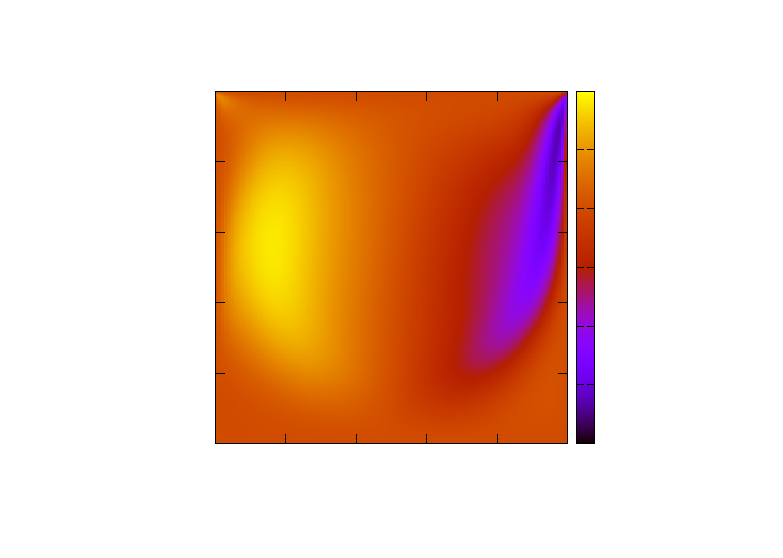
\includegraphics{DrivenCavity/Rv1000}}%
    \gplfronttext
  \end{picture}%
\endgroup
}
		\caption{$Re=1000$}
	\end{subfigure}
	\begin{subfigure}{0.5\textwidth}
		\resizebox{1.4\textwidth}{!}{% GNUPLOT: LaTeX picture with Postscript
\begingroup
  \makeatletter
  \providecommand\color[2][]{%
    \GenericError{(gnuplot) \space\space\space\@spaces}{%
      Package color not loaded in conjunction with
      terminal option `colourtext'%
    }{See the gnuplot documentation for explanation.%
    }{Either use 'blacktext' in gnuplot or load the package
      color.sty in LaTeX.}%
    \renewcommand\color[2][]{}%
  }%
  \providecommand\includegraphics[2][]{%
    \GenericError{(gnuplot) \space\space\space\@spaces}{%
      Package graphicx or graphics not loaded%
    }{See the gnuplot documentation for explanation.%
    }{The gnuplot epslatex terminal needs graphicx.sty or graphics.sty.}%
    \renewcommand\includegraphics[2][]{}%
  }%
  \providecommand\rotatebox[2]{#2}%
  \@ifundefined{ifGPcolor}{%
    \newif\ifGPcolor
    \GPcolortrue
  }{}%
  \@ifundefined{ifGPblacktext}{%
    \newif\ifGPblacktext
    \GPblacktexttrue
  }{}%
  % define a \g@addto@macro without @ in the name:
  \let\gplgaddtomacro\g@addto@macro
  % define empty templates for all commands taking text:
  \gdef\gplbacktext{}%
  \gdef\gplfronttext{}%
  \makeatother
  \ifGPblacktext
    % no textcolor at all
    \def\colorrgb#1{}%
    \def\colorgray#1{}%
  \else
    % gray or color?
    \ifGPcolor
      \def\colorrgb#1{\color[rgb]{#1}}%
      \def\colorgray#1{\color[gray]{#1}}%
      \expandafter\def\csname LTw\endcsname{\color{white}}%
      \expandafter\def\csname LTb\endcsname{\color{black}}%
      \expandafter\def\csname LTa\endcsname{\color{black}}%
      \expandafter\def\csname LT0\endcsname{\color[rgb]{1,0,0}}%
      \expandafter\def\csname LT1\endcsname{\color[rgb]{0,1,0}}%
      \expandafter\def\csname LT2\endcsname{\color[rgb]{0,0,1}}%
      \expandafter\def\csname LT3\endcsname{\color[rgb]{1,0,1}}%
      \expandafter\def\csname LT4\endcsname{\color[rgb]{0,1,1}}%
      \expandafter\def\csname LT5\endcsname{\color[rgb]{1,1,0}}%
      \expandafter\def\csname LT6\endcsname{\color[rgb]{0,0,0}}%
      \expandafter\def\csname LT7\endcsname{\color[rgb]{1,0.3,0}}%
      \expandafter\def\csname LT8\endcsname{\color[rgb]{0.5,0.5,0.5}}%
    \else
      % gray
      \def\colorrgb#1{\color{black}}%
      \def\colorgray#1{\color[gray]{#1}}%
      \expandafter\def\csname LTw\endcsname{\color{white}}%
      \expandafter\def\csname LTb\endcsname{\color{black}}%
      \expandafter\def\csname LTa\endcsname{\color{black}}%
      \expandafter\def\csname LT0\endcsname{\color{black}}%
      \expandafter\def\csname LT1\endcsname{\color{black}}%
      \expandafter\def\csname LT2\endcsname{\color{black}}%
      \expandafter\def\csname LT3\endcsname{\color{black}}%
      \expandafter\def\csname LT4\endcsname{\color{black}}%
      \expandafter\def\csname LT5\endcsname{\color{black}}%
      \expandafter\def\csname LT6\endcsname{\color{black}}%
      \expandafter\def\csname LT7\endcsname{\color{black}}%
      \expandafter\def\csname LT8\endcsname{\color{black}}%
    \fi
  \fi
    \setlength{\unitlength}{0.0500bp}%
    \ifx\gptboxheight\undefined%
      \newlength{\gptboxheight}%
      \newlength{\gptboxwidth}%
      \newsavebox{\gptboxtext}%
    \fi%
    \setlength{\fboxrule}{0.5pt}%
    \setlength{\fboxsep}{1pt}%
\begin{picture}(7200.00,5040.00)%
    \gplgaddtomacro\gplbacktext{%
    }%
    \gplgaddtomacro\gplfronttext{%
      \put(1908,624){\makebox(0,0){\strut{}$0$}}%
      \put(2585,624){\makebox(0,0){\strut{}$0.2$}}%
      \put(3262,624){\makebox(0,0){\strut{}$0.4$}}%
      \put(3938,624){\makebox(0,0){\strut{}$0.6$}}%
      \put(4615,624){\makebox(0,0){\strut{}$0.8$}}%
      \put(5292,624){\makebox(0,0){\strut{}$1$}}%
      \put(1720,938){\makebox(0,0)[r]{\strut{}$0$}}%
      \put(1720,1615){\makebox(0,0)[r]{\strut{}$0.2$}}%
      \put(1720,2292){\makebox(0,0)[r]{\strut{}$0.4$}}%
      \put(1720,2968){\makebox(0,0)[r]{\strut{}$0.6$}}%
      \put(1720,3645){\makebox(0,0)[r]{\strut{}$0.8$}}%
      \put(1720,4322){\makebox(0,0)[r]{\strut{}$1$}}%
      \put(5678,938){\makebox(0,0)[l]{\strut{}$-0.8$}}%
      \put(5678,1421){\makebox(0,0)[l]{\strut{}$-0.6$}}%
      \put(5678,1904){\makebox(0,0)[l]{\strut{}$-0.4$}}%
      \put(5678,2388){\makebox(0,0)[l]{\strut{}$-0.2$}}%
      \put(5678,2871){\makebox(0,0)[l]{\strut{}$0$}}%
      \put(5678,3355){\makebox(0,0)[l]{\strut{}$0.2$}}%
      \put(5678,3838){\makebox(0,0)[l]{\strut{}$0.4$}}%
      \put(5678,4322){\makebox(0,0)[l]{\strut{}$0.6$}}%
    }%
    \gplbacktext
    \put(0,0){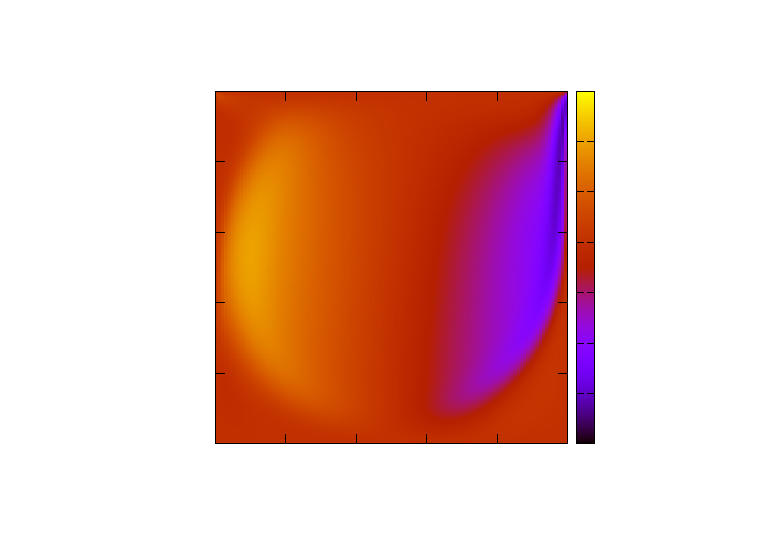
\includegraphics{DrivenCavity/Rv3200}}%
    \gplfronttext
  \end{picture}%
\endgroup
}
		\caption{$Re=3200$}
	\end{subfigure}%
	\begin{subfigure}{0.5\textwidth}
		\center
		\resizebox{1.4\textwidth}{!}{% GNUPLOT: LaTeX picture with Postscript
\begingroup
  \makeatletter
  \providecommand\color[2][]{%
    \GenericError{(gnuplot) \space\space\space\@spaces}{%
      Package color not loaded in conjunction with
      terminal option `colourtext'%
    }{See the gnuplot documentation for explanation.%
    }{Either use 'blacktext' in gnuplot or load the package
      color.sty in LaTeX.}%
    \renewcommand\color[2][]{}%
  }%
  \providecommand\includegraphics[2][]{%
    \GenericError{(gnuplot) \space\space\space\@spaces}{%
      Package graphicx or graphics not loaded%
    }{See the gnuplot documentation for explanation.%
    }{The gnuplot epslatex terminal needs graphicx.sty or graphics.sty.}%
    \renewcommand\includegraphics[2][]{}%
  }%
  \providecommand\rotatebox[2]{#2}%
  \@ifundefined{ifGPcolor}{%
    \newif\ifGPcolor
    \GPcolortrue
  }{}%
  \@ifundefined{ifGPblacktext}{%
    \newif\ifGPblacktext
    \GPblacktexttrue
  }{}%
  % define a \g@addto@macro without @ in the name:
  \let\gplgaddtomacro\g@addto@macro
  % define empty templates for all commands taking text:
  \gdef\gplbacktext{}%
  \gdef\gplfronttext{}%
  \makeatother
  \ifGPblacktext
    % no textcolor at all
    \def\colorrgb#1{}%
    \def\colorgray#1{}%
  \else
    % gray or color?
    \ifGPcolor
      \def\colorrgb#1{\color[rgb]{#1}}%
      \def\colorgray#1{\color[gray]{#1}}%
      \expandafter\def\csname LTw\endcsname{\color{white}}%
      \expandafter\def\csname LTb\endcsname{\color{black}}%
      \expandafter\def\csname LTa\endcsname{\color{black}}%
      \expandafter\def\csname LT0\endcsname{\color[rgb]{1,0,0}}%
      \expandafter\def\csname LT1\endcsname{\color[rgb]{0,1,0}}%
      \expandafter\def\csname LT2\endcsname{\color[rgb]{0,0,1}}%
      \expandafter\def\csname LT3\endcsname{\color[rgb]{1,0,1}}%
      \expandafter\def\csname LT4\endcsname{\color[rgb]{0,1,1}}%
      \expandafter\def\csname LT5\endcsname{\color[rgb]{1,1,0}}%
      \expandafter\def\csname LT6\endcsname{\color[rgb]{0,0,0}}%
      \expandafter\def\csname LT7\endcsname{\color[rgb]{1,0.3,0}}%
      \expandafter\def\csname LT8\endcsname{\color[rgb]{0.5,0.5,0.5}}%
    \else
      % gray
      \def\colorrgb#1{\color{black}}%
      \def\colorgray#1{\color[gray]{#1}}%
      \expandafter\def\csname LTw\endcsname{\color{white}}%
      \expandafter\def\csname LTb\endcsname{\color{black}}%
      \expandafter\def\csname LTa\endcsname{\color{black}}%
      \expandafter\def\csname LT0\endcsname{\color{black}}%
      \expandafter\def\csname LT1\endcsname{\color{black}}%
      \expandafter\def\csname LT2\endcsname{\color{black}}%
      \expandafter\def\csname LT3\endcsname{\color{black}}%
      \expandafter\def\csname LT4\endcsname{\color{black}}%
      \expandafter\def\csname LT5\endcsname{\color{black}}%
      \expandafter\def\csname LT6\endcsname{\color{black}}%
      \expandafter\def\csname LT7\endcsname{\color{black}}%
      \expandafter\def\csname LT8\endcsname{\color{black}}%
    \fi
  \fi
    \setlength{\unitlength}{0.0500bp}%
    \ifx\gptboxheight\undefined%
      \newlength{\gptboxheight}%
      \newlength{\gptboxwidth}%
      \newsavebox{\gptboxtext}%
    \fi%
    \setlength{\fboxrule}{0.5pt}%
    \setlength{\fboxsep}{1pt}%
\begin{picture}(7200.00,5040.00)%
    \gplgaddtomacro\gplbacktext{%
    }%
    \gplgaddtomacro\gplfronttext{%
      \csname LTb\endcsname%
      \put(1908,624){\makebox(0,0){\strut{}$0$}}%
      \put(2585,624){\makebox(0,0){\strut{}$0.2$}}%
      \put(3262,624){\makebox(0,0){\strut{}$0.4$}}%
      \put(3938,624){\makebox(0,0){\strut{}$0.6$}}%
      \put(4615,624){\makebox(0,0){\strut{}$0.8$}}%
      \put(5292,624){\makebox(0,0){\strut{}$1$}}%
      \put(1720,938){\makebox(0,0)[r]{\strut{}$0$}}%
      \put(1720,1615){\makebox(0,0)[r]{\strut{}$0.2$}}%
      \put(1720,2292){\makebox(0,0)[r]{\strut{}$0.4$}}%
      \put(1720,2968){\makebox(0,0)[r]{\strut{}$0.6$}}%
      \put(1720,3645){\makebox(0,0)[r]{\strut{}$0.8$}}%
      \put(1720,4322){\makebox(0,0)[r]{\strut{}$1$}}%
      \put(5678,938){\makebox(0,0)[l]{\strut{}$-0.7$}}%
      \put(5678,1245){\makebox(0,0)[l]{\strut{}$-0.6$}}%
      \put(5678,1553){\makebox(0,0)[l]{\strut{}$-0.5$}}%
      \put(5678,1860){\makebox(0,0)[l]{\strut{}$-0.4$}}%
      \put(5678,2168){\makebox(0,0)[l]{\strut{}$-0.3$}}%
      \put(5678,2476){\makebox(0,0)[l]{\strut{}$-0.2$}}%
      \put(5678,2783){\makebox(0,0)[l]{\strut{}$-0.1$}}%
      \put(5678,3091){\makebox(0,0)[l]{\strut{}$0$}}%
      \put(5678,3399){\makebox(0,0)[l]{\strut{}$0.1$}}%
      \put(5678,3706){\makebox(0,0)[l]{\strut{}$0.2$}}%
      \put(5678,4014){\makebox(0,0)[l]{\strut{}$0.3$}}%
      \put(5678,4322){\makebox(0,0)[l]{\strut{}$0.4$}}%
    }%
    \gplbacktext
    \put(0,0){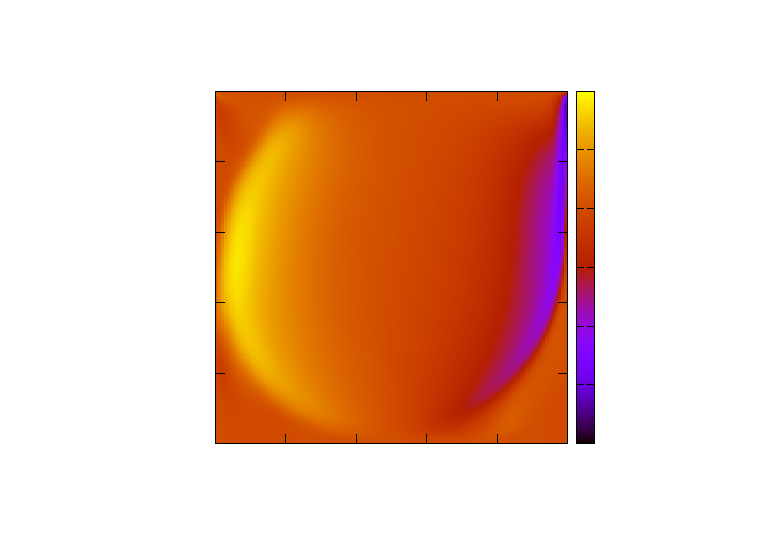
\includegraphics{Rv10000}}%
    \gplfronttext
  \end{picture}%
\endgroup
}
		\caption{$Re=10000$}
	\end{subfigure}
	\caption{Vertical velocity in the cavity}
	\label{DrivenVerticalDomain}
\end{figure}

For the vertical velocities (figure \ref{DrivenVerticalDomain}) the behaviour is similar to that of the horizontal velocities. For low Re, there is only velocity in the top of the vertical walls. However, as the Re increases, the region with vertical velocity also increases, showing again the distribution of a clockwise rotation. The gradient of velocities in the right wall is stronger for higher Reynolds numbers. In the case of $Re=10000$ the distribution shows that the region with vertical velocity stretches, but these results may not be accurate.

As a conclusion, for lower Reynolds numbers, viscosity only allows a small movement in the upper region of the cavity. This is the case of $Re=100$. But for higher Re, inertial forces become more important and the behaviour of the flow is completely different. The fluid starts to rotate around the centre of the cavity. As the Re increases, the motion becomes more complex and other small vortices appear in the sides of the cavity.

%\subsection{Streamlines}
%In order to know the distribution of the velocity along the cavity, it i useful to plot the streamlines of the flow. They are defined by the stream function $\psi$:
%\begin{equation}
%\frac{\partial\psi}{\partial x}=-v
%\qquad\qquad
%\frac{\partial\psi}{\partial y}=u
%\end{equation}
%A streamline is a line everywhere tangent to the velocity vector at a given instant:
%\begin{equation}
%\frac{dx}{u}=\frac{dy}{v}
%\end{equation}
%Combining both expressions \cite{Haegland2007}:
%\begin{equation}
%\psi\left(x, y\right)=\int udy-\int vdx+\int\left(\int\frac{dv}{dy}dx\right)dy
%\end{equation}